 %
% File acl2021.tex
%
%% Based on the style files for EMNLP 2020, which were
%% Based on the style files for ACL 2020, which were
%% Based on the style files for ACL 2018, NAACL 2018/19, which were
%% Based on the style files for ACL-2015, with some improvements
%%  taken from the NAACL-2016 style
%% Based on the style files for ACL-2014, which were, in turn,
%% based on ACL-2013, ACL-2012, ACL-2011, ACL-2010, ACL-IJCNLP-2009,
%% EACL-2009, IJCNLP-2008...
%% Based on the style files for EACL 2006 by 
%%e.agirre@ehu.es or Sergi.Balari@uab.es
%% and that of ACL 08 by Joakim Nivre and Noah Smith

\documentclass[11pt,a4paper]{article}
\usepackage[hyperref]{acl2021}
\usepackage{times}
\usepackage{latexsym}
\usepackage{graphicx}
\usepackage{caption}
\usepackage{float}
\usepackage{amsmath}
\usepackage{amssymb}
\usepackage{booktabs}
\usepackage{tabularx}
\usepackage{array}
\usepackage{multirow}
\usepackage{graphicx}
\usepackage{algorithm}
\usepackage{algpseudocode}
\usepackage{tcolorbox}
\tcbuselibrary{most}
\usepackage{enumitem}
\usepackage{multicol}
\usepackage{tikz}
\usepackage{bbm}
\usepackage{microtype}
\usepackage{lmodern}
\usepackage[T1]{fontenc}

% \usepackage{subcaption} % optional, if you want side-by-side images

\renewcommand{\UrlFont}{\ttfamily\small}

% This is not strictly necessary, and may be commented out,
% but it will improve the layout of the manuscript,
% and will typically save some space.
\usepackage{microtype}

\aclfinalcopy % Uncomment this line for the final submission
%\def\aclpaperid{***} %  Enter the acl Paper ID here

%\setlength\titlebox{5cm}
% You can expand the titlebox if you need extra space
% to show all the authors. Please do not make the titlebox
% smaller than 5cm (the original size); we will check this
% in the camera-ready version and ask you to change it back.

\newcommand\BibTeX{B\textsc{ib}\TeX}

\title{Incentivizing both Grounding and Reasoning in Large Language Models with Online Reinforcement Learning}

\author{
  Pavanpreet Singh Gandhi, Julian Ma, Xu Chen, Michael Yiu \\
  Department of Computer Science, University College London \\
  \texttt{\{pavanpreet.gandhi.24, julian.ma.24, xu.chen.24, chun.yiu.24\}@ucl.ac.uk}\\ 
}

\date{}

\begin{document}
\thispagestyle{plain}
\pagestyle{plain}
\maketitle
\begin{abstract}
    We investigate whether prompting LLM agents to reason before action selection 
    improves sample efficiency and generalization during online reinforcement learning in BabyAI-Text environments. 
    Unlike prior approaches, our method allows LLMs to generate actions token-by-token with a nested RL approach that attributes rewards 
    across the decision process. 
    Comparing agents prompted to reason before acting against those generating actions directly, 
    we find explicit reasoning does not consistently yield performance advantages, 
    with both agent types achieving comparable success rates after PPO fine-tuning. 
    We identify a ``reasoning collapse'' phenomenon where agents occasionally simply state actions without providing thought processes. 
    While reasoning agents exhibited similar performance to direct-action agents, they showed greater training instability. 
    Our findings suggest explicit reasoning offers valuable interpretability without compromising effectiveness, 
    contributing to understanding the interplay between reasoning, grounding, and reinforcement learning in LLM-based agents\footnote{Our source code can be found in \url{https://github.com/pavanpreet-gandhi/rl-llm}}.
\end{abstract}

\section{Introduction}
Large Language Models (LLMs) have demonstrated promising capabilities in sequential decision-making problems \cite{yao2023treethoughtsdeliberateproblem, yao2023react}, leveraging pre-trained knowledge to navigate environments without task-specific fine-tuning \cite{wang2023voyager}. However, trained primarily on next-token prediction, LLMs lack a \textit{grounded} understanding of environment dynamics—they cannot reliably map tokens to actions, anticipate states, or comprehend reward implications. Recent research \cite{carta2023grounding} addresses this limitation through online reinforcement learning (RL) to improve grounding.

On the other hand, RL has emerged as a method for enhancing LLMs by aligning with human preferences \cite{ouyang2022training} and incentivizing reasoning capabilities \cite{deepseek2025r1, lambert2024t}. Yet the combination of reasoning and online RL for grounding LLMs in sequential decision-making remains relatively unexplored.

We investigate whether explicit reasoning during online RL fine-tuning improves LLM-based agents' performance. Using BabyAI-Text \cite{carta2023grounding}, we compare (1) agents prompted to reason before action selection, and (2) agents generating actions directly without reasoning steps. Unlike prior work \cite{carta2023grounding}, our approach allows token-by-token action generation rather than selection from predefined options. We hypothesized reasoning-enabled agents would demonstrate superior sample efficiency and generalization to novel tasks.
Our results reveal that explicit reasoning provides no consistent performance advantage over direct action generation, with both approaches achieving comparable success rates after PPO fine-tuning. Furthermore, reasoning agents sometimes exhibit greater training instability and occasionally a ``reasoning collapse'' phenomenon where explanatory text devolved into simply stating the intended action. Nevertheless, when they work, reasoning-based agents offered valuable interpretability benefits without compromising effectiveness.

\section{Related Work}
\subsection{LLM Reasoning}
LLM reasoning capabilities have seen substantial advances through both supervised prompting and reinforcement learning. A foundational idea is Chain-of-Thought (CoT) prompting \cite{wei2022chain}, where LLMs are prompted to articulate intermediate reasoning steps to improve performance on arithmetic and commonsense tasks. This idea is further refined in Self-Consistency \cite{wang2022self}, which samples multiple CoT paths and selects the most coherent solution and in Tree of Thoughts \cite{yao2023treethoughtsdeliberateproblem} where multiple reasoning paths are evaluated before final output. Similarly, Scratchpad-style reasoning \cite{nye2021show} encourages LLMs to generate and retain intermediate states during problem solving, improving interpretability and generalization; while Reflexion \cite{shinn2023reflexion} proposed a framework to allow LLMs to verbally reflect on task feedback signals which are then maintained in a memory buffer to improve decision making.

Other works leverage reinforcement learning to enhance reasoning. RLHF \cite{ouyang2022training} adapts PPO to fine-tune model outputs from human preferences, while DeepSeek-R1 \cite{deepseek2025r1} and TULU-3 \cite{lambert2024t} leverage reinforcement learning and verifiable rewards to incentivise reasoning capabilities. VinePPO \cite{kazemnejad2024vineppo} proposes a PPO variant that replaces the value network with Monte Carlo rollouts for intermediate steps, directly supporting reasoning processes. Recent efforts like STaR \cite{zelikman2022star} introduce iterative self-training to refine CoT traces over time, demonstrating that LLMs can bootstrap their own reasoning with minimal supervision.

More structured paradigms have also emerged. Towards System 2 Reasoning \cite{xiang2025towards} extends CoT via explicit modeling of the underlying reasoning (``Meta-CoT'') and explored methods including process supervision, synthetic data generation and search algorithms. Cognitive Behaviors for Self-Improving Reasoners \cite{gandhi2025cognitive} identifies four key strategies—verification, backtracking, subgoal setting, and backward chaining—that are critical for performance improvements in RL training. 

Collectively, these studies highlight the importance of structured, interpretable reasoning in LLMs. In our work, we evaluate the effect of prompting the agent to explicitly reason before generating actions, with the goal of improving sample efficiency and generalization in BabyAI-Text environments.

\subsection{LLM Agents}

A growing body of work investigates how LLMs can be adapted into interactive agents capable of grounding language into actions. These agents must interpret instructions, model the world, and make decisions based on partially observable environments. GLAM \cite{carta2023grounding} demonstrates that grounded LLMs, when trained with PPO in BabyAI-text environments, achieve both strong task performance and high sample efficiency. Our work is closely related to GLAM, but we extend it by prompting the agent to explicitly reason before generating actions.

Others explore how LLMs can operate as agents by tightly coupling reasoning and action. ReAct \cite{yao2023react} interleaves ``thoughts'' and ``acts'' during each step, showing that such interleaving improves success rates in interactive decision-making tasks. Inner Monologue \cite{huang2022inner} applies this idea to robotics, allowing agents to maintain internal self-dialogue to better interpret sensor inputs and act appropriately. Although its domain differs from ours, the notion of internal reasoning aligns with our reasoning-before-acting policy design.

Language Models as Zero-Shot Planners \cite{huang2022language} illustrates that pretrained models such as GPT-3 can compose multi-step symbolic plans without environment interaction or gradient updates, relying on latent world knowledge. SayCan \cite{ahn2022can} adds an external value function to verify action feasibility, demonstrating the effectiveness of combining LLMs with decision-checking mechanisms — a strategy structurally similar to our use of value heads trained via PPO.

Recent works have expanded the scope of LLMs as agents by introducing real-world affordances and grounding. Language Models can Solve Computer Tasks \cite{kim2023language} shows that LLMs can control a simulated computer environment to solve programming and OS-level tasks, learning to act through API interfaces. Meanwhile, Language Models Meet World Models \cite{xiang2023language} investigates how interaction with embodied world models — even simulated ones — improves reasoning and task completion, arguing that LLMs benefit from experiential learning.

To enhance LLM agency in multimodal or partially grounded environments, Grounding Multimodal Large Language Models in Actions \cite{szot2024grounding} trains models that integrate language, vision, and proprioception. The authors show that with sufficient alignment, these models can directly translate instructions into physical actions, highlighting the importance of reward-aligned updates and latent action representations — themes echoed in our own use of PPO and value modeling for action refinement.

Other frameworks such as Voyager \cite{wang2023voyager} use LLMs to autonomously explore and craft tools in Minecraft, Toolformer \cite{schick2023toolformer} use LLM to interact with external tools using APIs while LOOP \cite{chen2025reinforcement} and Learning to Search in Language \cite{gandhi2024stream} enable agents to iteratively improve their plans by simulating search processes in natural language. These systems represent a shift from prompt-only agents to learning systems that adapt through interaction, long-term memory, or reinforcement.

These works point toward a convergence between LLMs and traditional agentic systems. 
Through reinforcement learning, interaction, and grounding, 
LLMs are increasingly capable of planning, adapting, and acting in dynamic environments. 
Our study contributes further by examining how reasoning affects sample efficiency and policy generalization in a text-based BabyAI environment.

\section{Methods}

\subsection{Environment: BabyAI-Text}
BabyAI-Text \cite{carta2023grounding} is a textual extension of the BabyAI platform \cite{chevalier2018babyai} designed to study functional grounding of language models in interactive environments. 
It replaces the original symbolic observations of BabyAI with natural language descriptions, enabling interaction through a text-only interface. 
The environment retains the procedurally generated minigrid setup and low-level navigation tasks, while providing language-based goals and observations. 
Agents must interpret textual inputs, reason about spatial configurations, and execute actions like ``go forward'' or ``pick up'' to achieve sparse reward objectives.  
An example interaction is shown in Appendix \ref{appendix: babyai-text}.

We systematically vary environment complexity by introducing different quantities of distractor objects (0, 3, or 5) 
that the agent must navigate around or distinguish from target objects. 
These distractors create more complex spatial configurations and increase the perceptual load, 
requiring the agent to filter relevant information from observations.

The reward structure is sparse and goal-driven: the agent receives a positive reward (maximum +1) 
only upon successful task completion, with higher values for faster completion. 
Most intermediate steps yield zero reward, except for invalid actions which incur a -1 penalty. 
This sparse, delayed reward signal presents a challenging credit assignment problem, 
motivating our nested reinforcement learning approach as described in Section \ref{subsec: PPO-based-LLM-fine-tuning}.

\subsection{Prompt Design and Action Output}
\label{subsec: 3.4}
To investigate how explicit reasoning affects the performance and sample efficiency of the LLM agent, we designed two different prompting strategies for the agent's action output:

\paragraph{Direct Action (No Reasoning)} 
In this approach, the agent is prompted to output only a valid action command without additional commentary. The LLM's response at each time step is simply an environment action (e.g., ``pick up'') in free-form text. This setup treats the LLM purely as a policy $\pi(a|s)$, mapping observations and instructions directly to actions, analogous to standard RL agents. The full prompt is provided in Appendix \ref{appendix:prompts}.

\paragraph{Reasoning}
For the reasoning variant, the prompt encourages the agent to articulate a brief ``thought'' process before outputting the action. The prompt suggests limiting reasoning to ``at most 10 words'', though this is not enforced as a hard limit but rather a guideline to prevent excessively long reasoning chains for computational reasons. For example, an agent might respond: \textit{``The key is needed first. final answer: pick up''}. The text preceding \textit{``final answer:''} represents the agent's internal reasoning, which is ignored by the environment; only the action specified after the delimiter is executed.

In both modes, the context provided to the LLM includes the initial mission instruction and a history of previous observations and actions. Critically, when the agent produces an invalid response, we replace it in the context window with a warning message rather than preserving the original text. This design choice proved essential for training stability, as invalid responses often contain nonsensical characters that can trigger negative feedback loops where the model continues to produce similar invalid outputs. By sanitizing the context window in this way, we prevent the model from being influenced by its own previously invalid responses. More details on context window management and handling of invalid responses are provided in Appendices \ref{appendix:invalid_action} and \ref{appendix:chat_template}.

\subsection{PPO-Based LLM Fine-tuning}
\label{subsec: PPO-based-LLM-fine-tuning}

Following Carta et al.'s GLAM method \cite{carta2023grounding}, we employ Proximal Policy Optimization (PPO) \cite{schulman2017proximal} to fine-tune the LLM's policy. 
Unlike GLAM, which computes conditional probabilities for each action, our approach allows the model to generate free-form responses, and we extend this framework even further to integrate explicit reasoning during training.

Our policy is based on LLaMA-3.2-3B-Instruct (chosen for its performance in preliminary tests; see Appendix \ref{appendix:choice_of_baseline}), 
augmented with a small value head (single linear layer applied to the final hidden state) that estimates state value $V_\phi(s_t, y_t^{1:m-1})$, where $s_t$ is the query sequence at $t$ and $y_t^{1:m-1}$ are the response sequence before token $y_t^m$.
During PPO training, this value head is updated to minimise the mean-squared error to the empirical returns, 
while the policy parameters are updated by maximising the PPO clipped objective.
We use a KL-divergence penalty to keep the policy close to pretrained distributions and employ Low-Rank Adaptation (LoRA) \cite{hu2021lora} for parameter-efficient fine-tuning.

Training LLM agents introduces a critical challenge: reconciling the nested nature of environment interaction and token generation. 
The agent operates simultaneously in two distinct loops with different granularity of observation, action, and reward. 
In the environment loop, the agent processes textual descriptions of the environment state and produces valid commands (e.g., ``turn left'', ``go forward''). 
Rewards are typically sparse and often delayed until task completion. 
This loop represents the traditional reinforcement learning scenario where the agent's objective is to maximize cumulative environmental rewards. 
Meanwhile, within each environment step, the token generation loop unfolds as the LLM auto-regressively produces individual tokens conditioned on the context, history, and partial outputs. 
Each token prediction constitutes an LLM action drawn from the model's vocabulary, and the tokens themselves make up the environment action.
The challenge lies in appropriately attributing credit from sparse environment rewards to individual token predictions.

Our nested-loop challenge is addressed using a dual-level credit assignment approach. Algorithm \ref{alg:ppo} details our nested PPO training implementation. To regularize training, we incorporate penalty-free future returns while restricting penalties to immediate TD returns, see more details in Appendix \ref{appendix:ppo_comp}. Training hyperparameters are fully documented in Appendix \ref{appendix:hyperparameter}.

For comparison, Transformer Reinforcement Learning's \texttt{PPOTrainer}\footnote{\url{https://huggingface.co/docs/trl/en/ppo\_trainer}} implements language-based PPO where query-response pairs receive scalar scores. This approach is more akin to contextual bandits where all the environment level (outer loop) actions recieve the same reward which is the final reward of the episode, which proves unsuitable for our task by neglecting autocorrelation in sequential environment interactions. We validate our algorithm choice through comparative analysis with \texttt{PPOTrainer} in Appendix \ref{appendix:ppo_comp}. 

\begin{algorithm*}
\caption{Nested PPO Training Loops for LLM's}
\begin{algorithmic}[1]
\State \textbf{Input:} Initial token generation policy parameters $\theta$, value function parameters $\phi$, learning rate $\eta$, number of iterations $K$
\For{$k = 1$ to $K$}
    \State Collect $N$ trajectories $(s_1, y_1, r_2, s_2, y_2, r_3, \dots, r_T)$ using policy $\pi_\theta$
    \For{each timestep $t = T$ to $1$ in a trajectory}
        \State Compute penalty-free future TD($\lambda$) return
        \[\hat{G}_{t+1} = \mathrm{max}(0, r_{t+2}) + \gamma((1-\lambda)V_\phi(s_{t+1}, y_{t+1}) + \lambda \hat{G}_{t+2}^\lambda)\]
        \State Compute TD($\lambda$) return
        \[G_t^\lambda = r_{t+1} + \gamma((1-\lambda)V_\phi(s_t, y_t) + \lambda \hat{G}_{t+1}^\lambda)\]
        \For{each token $m = 1$ to $M$}
            \State Compute KL
            \[\mathrm{KL}_t^m \;=\; \log \pi_\theta\bigl(y^m_t \mid x^m_t\bigr) \;-\; \log \pi_{\text{ref}}\bigl(y^m_t \mid x^m_t\bigr),\;\;\;\;x^m_t := (s_t, y^{1:m-1}_t)\]
            \State Compute final reward for each token
            \[R^m_t \;=\; \mathbbm{1}\{m=M\} \cdot G_t^\lambda \;-\; \beta \,\mathrm{KL}^m_t\]
            \State Compute TD residual
            \[
            \delta^m_t = R^{m+1}_{t} + \gamma_{\text{token}}V_\phi(s_{t}, y_{t}^{m+1}) - V_\phi(s_t, y_t^m)
            \]
            \State Compute GAE on sequence
            \[
                \hat{A}^m_t = \delta^m_t + (\gamma_{\text{token}}\lambda_{\text{token}})\hat{A}_t^{m+1}\;\;\;\;\;\hat{A}_t^M = 0
            \]
        \EndFor
    \EndFor
    \State Update policy $\pi_\theta$ by maximizing $\mathcal{L}^{\mathrm{CLIP}}(\theta)$ via gradient ascent
    \[
    \mathcal{L}^{\mathrm{CLIP}}(\theta) = \mathbb{E}_t \left[ 
\min\left(\frac{\pi_\theta(a_t|s_t)}{\pi_{\theta_{\text{old}}}(a_t|s_t)}\,\hat{A}_t, \mathrm{clip}(r_t(\theta),\, 1{-}\epsilon,\, 1{+}\epsilon)\,\hat{A}_t \right) \right],
    \]
    \State Update value function $V_\phi$ by minimizing 
    \[
    \frac{1}{2}\sum\big(V_\phi(s_t, y_t) - G_t^{\lambda}\big)^2
    \]
\EndFor
\end{algorithmic}
\label{alg:ppo}
\end{algorithm*}

\section{Experiments}
To evaluate our hypothesis regarding the benefits of explicit reasoning during reinforcement learning, 
we conducted a series of controlled experiments across 10 distinct training runs.
For all experiments, we used ``go to'' and ``pick up'' tasks in the BabyAI-Text environment, 
because GLAM \cite{carta2023grounding} has shown that these tasks are simple enough for LLMs to learn quickly.
We established three environment configurations with increasing levels of complexity:
(1) \textbf{0 distractors}: The agent must navigate to (or pick up) a single target object;
(2) \textbf{3 distractors}: The agent must navigate with three randomly placed distractor objects; and
(3) \textbf{5 distractors}: The agent must navigate with five distractor objects.
Among all experiments, the only variables that differ are the number of distractors and the reasoning mechanism.
All other hyperparameters, are kept constant as described in Table \ref{appendix:hyperparameter} in the appendix.
\subsection{Performance Across Environment Configurations}
\label{subsec: 4.1}
For each configuration, we trained both reasoning and non-reasoning agents while maintaining consistent hyperparameters.
We show the success rate and average reward of batches of episodes collected during training for the three-distractor case in Figure \ref{fig:three_distractors} and for the zero and five distractor cases in Appendix \ref{appendix: training-curves}.

In the simplest environment without distractors (Fig. \ref{fig:no_distractors}), non-reasoning agents achieved perfect success rates (1.0) from the beginning of training, 
demonstrating effective zero-shot transfer. Reasoning agents initially struggled with generating valid actions but eventually converged to perfect success rates.
The mixed results in average reward metrics suggest that in simple environments, 
explicit reasoning does not provide any significant advantage over the non-reasoning agent.

With three distractors (Fig. \ref{fig:three_distractors}), we observed one reasoning agent outperform the non-reasoning agents in terms of average reward, 
while the other reasoning agent experienced unstable training and had to be terminated early.
This instability was not observed in non-reasoning agents and required special mitigation techniques discussed in Appendix \ref{appendix:invalid_action}.

\begin{figure*}[t]
    \centering
    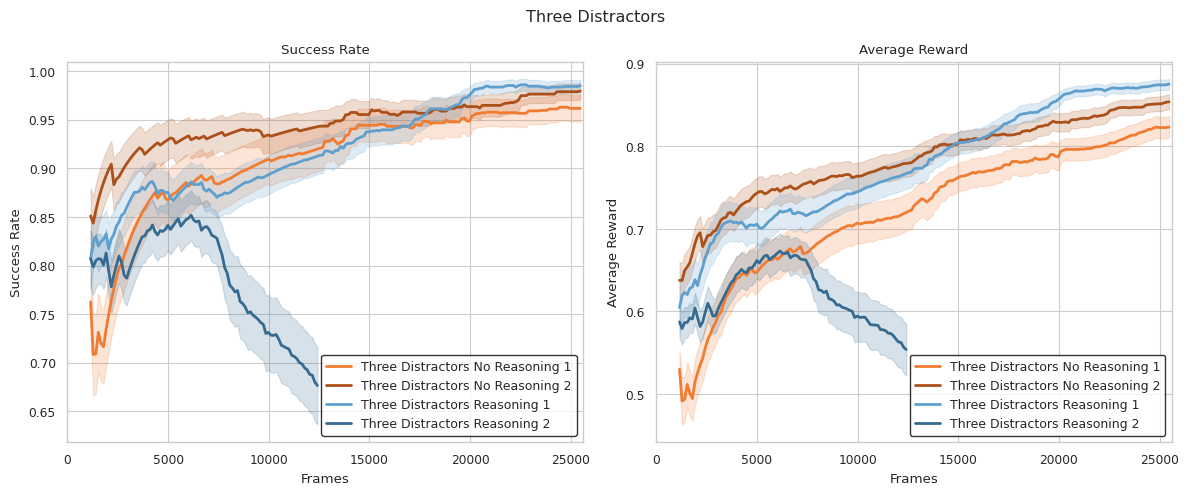
\includegraphics[width=\textwidth]{../images/three_distractors_training_curves.png}
    \caption{Training curves for agents in environments with three distractors.}
    \label{fig:three_distractors}
\end{figure*}

In the most difficult configuration with five distractors (Fig. \ref{fig:five_distractors}), 
both reasoning and non-reasoning agents demonstrated comparable performance in terms of success rates and average rewards.

\subsection{Reasoning Collapse}
We identified an intriguing pattern during training that we term ''reasoning collapse'', 
where agents' explicit reasoning simply states the action they are about to take rather than providing a coherent thought process.
Normally, reasoning agents produced coherent thoughts before actions, as shown:
\begin{tcolorbox}[
    enhanced,
    title={Normal Reasoning Example},
    fonttitle=\bfseries,
    colback=gray!10,
    colframe=black!50,
    boxrule=0.5pt,
    arc=2pt,
    outer arc=2pt,
    top=2pt,
    bottom=2pt,
    left=4pt,
    right=4pt,
    boxsep=2pt
]
\textbf{Observation:}

You see a wall 2 steps right

You see a blue key 3 steps left and 1 step forward

You see a yellow key 2 steps forward

\textbf{Agent Response:}

I should go forward to get slightly closer to the blue key.

final answer: go forward
\end{tcolorbox}
However, as training progressed, we observed instances where reasoning text simply stated the action:
\begin{tcolorbox}[
    enhanced,
    title={Collapsed Reasoning Example},
    fonttitle=\bfseries,
    colback=gray!10,
    colframe=black!50,
    boxrule=0.5pt,
    arc=2pt,
    outer arc=2pt,
    top=2pt,
    bottom=2pt,
    left=4pt,
    right=4pt,
    boxsep=2pt
]
\textbf{Observation:}

You see a wall 2 steps forward

You see a wall 3 steps right

You see a purple key 3 steps left

You see a blue key 2 steps left and 1 step forward

\textbf{Agent Response:}

Go forward.

final answer: go forward
\end{tcolorbox}

Figure \ref{fig:reasoning_length} displays the average reasoning text length for the 3-distractor environment, 
with similar patterns observed across all runs. 
The text length shows high variability throughout training, 
frequently collapsing to just two words. 
Later training batches typically contain both normal and collapsed reasoning outputs. 
This phenomenon suggests either that (1) the agent discovers explicit reasoning isn't necessary for maximizing rewards, 
or (2) reasoning processes become internalized within the model's latent representations as training advances.

\begin{figure*}[t]
    \centering
    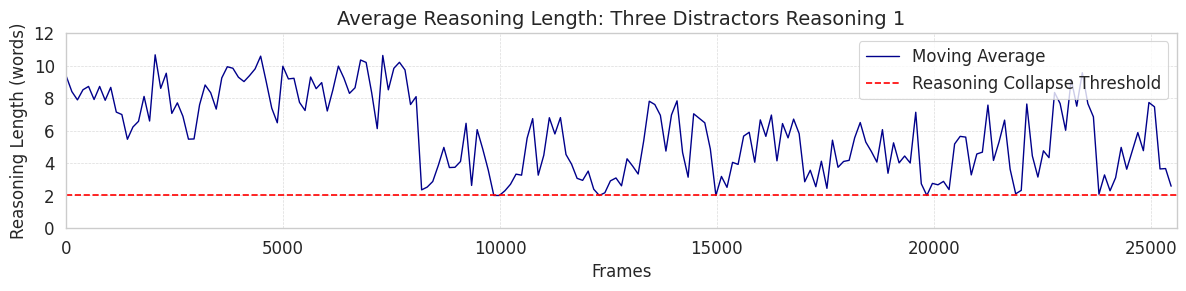
\includegraphics[width=0.8\textwidth]{../images/avg_reasoning_length_three_distractors_reasoning_1.png}
    \caption{Average length of reasoning text (in words) generated by the reasoning agent over time during training in the 3-distractor environment.}
    \label{fig:reasoning_length}
\end{figure*}

\section{Results and Discussion}
\subsection{Evaluation Results}
We evaluated both trained and untrained models across three distinct task environments -- varying in environment complexity with 0, 3 and 5 distractors -- and compared the two prompting strategies outlined in Section \ref{subsec: 3.4}. Each envrionment configuration was assessed using four BabyAI tasks: \texttt{GoTo}, \texttt{Pickup}, \texttt{GoToTest} and \texttt{PickupTest}. Performance metrics used include success rate and average reward. The detailed evaluation results for the environment setting with 3 distractors can be found in Table \ref{tab:performance3}, while those from environment setting with 0 and 5 distractors, as well as visualisations of these performance metrics can found in Appendix \ref{app:F}. We also evaluated our models' performance on benchmarks outside of BabyAI-Text and found no clear difference between reasoning and non-reasoning models Appendix \ref{app:Z}.

\begin{table*}[t]
\centering
\scriptsize
\begin{tabularx}{\linewidth}{%
    l l
    >{\centering\arraybackslash}X 
    >{\centering\arraybackslash}X 
    >{\centering\arraybackslash}X 
    >{\centering\arraybackslash}X }
\toprule
\textbf{Env} & \textbf{Model Variant} 
& \textbf{Reasoning Success Rate $\pm$ Std} 
& \textbf{Non-Reasoning Success Rate $\pm$ Std} 
& \textbf{Reasoning Avg Reward $\pm$ Std} 
& \textbf{Non-Reasoning Avg Reward $\pm$ Std} \\
\midrule
\multirow{3}{*}{GoTo-v0} 
    & Zero-shot                & $0.46\pm0.50$ & $0.80\pm0.40$ & $0.34\pm0.41$ & $0.53\pm0.34$ \\
    & Three-Distractor\_1     & $0.98\pm0.14$ & $0.98\pm0.14$ & $0.88\pm0.15$ & $0.86\pm0.16$ \\
    & Three-Distractor\_2     & $0.14\pm0.35$ & $1.00\pm0.00$ & $0.13\pm0.33$ & $0.89\pm0.08$ \\
\midrule
\multirow{3}{*}{Pickup-v0} 
    & Zero-shot                & $0.18\pm0.39$ & $0.42\pm0.50$ & $0.12\pm0.28$ & $0.30\pm0.38$ \\
    & Three-Distractor\_1     & $0.96\pm0.20$ & $0.74\pm0.44$ & $0.86\pm0.19$ & $0.63\pm0.40$ \\
    & Three-Distractor\_2     & $0.22\pm0.42$ & $0.82\pm0.39$ & $0.20\pm0.38$ & $0.68\pm0.34$ \\
\midrule
\multirow{3}{*}{GoToTest-v0} 
    & Zero-shot                & $0.62\pm0.49$ & $0.86\pm0.35$ & $0.48\pm0.41$ & $0.62\pm0.33$ \\
    & Three-Distractor\_1     & $1.00\pm0.00$ & $0.98\pm0.14$ & $0.91\pm0.08$ & $0.85\pm0.16$ \\
    & Three-Distractor\_2     & $0.20\pm0.40$ & $1.00\pm0.00$ & $0.19\pm0.39$ & $0.90\pm0.07$ \\
\midrule
\multirow{3}{*}{PickupTest-v0} 
    & Zero-shot                & $0.28\pm0.45$ & $0.38\pm0.49$ & $0.19\pm0.33$ & $0.27\pm0.37$ \\
    & Three-Distractor\_1     & $0.92\pm0.27$ & $0.82\pm0.39$ & $0.80\pm0.26$ & $0.73\pm0.35$ \\
    & Three-Distractor\_2     & $0.10\pm0.30$ & $0.72\pm0.45$ & $0.08\pm0.26$ & $0.60\pm0.39$ \\
\bottomrule
\end{tabularx}
\caption{Per-variant performance of reasoning and non-reasoning models in environments with three distractors.}
\label{tab:performance3}
\end{table*}

\subsection{Discussion}
\paragraph{Zero-distractor Environment}
Table \ref{tab:performance0} in Appendix \ref{app:F} summarises the performance metrics for both the zero-shot models and the models trained in this environment. In the simplest setting with no distractors, the zero-shot baseline without reasoning achieved a high success rate of 94\%, while the reasoning-enabled baseline performed notably worse at 66\%, likely due to the additional output formatting constraints and the complexity of reasoning generation. After training, both reasoning and non-reasoning agents consistently achieved 100\% success rates, with only minor differences in average rewards and episode lengths. This confirms that, explicit reasoning does not yield tangible performance benefits in simple environments, and it imposes an initial learning overhead -- namely, the need to learn to structure outputs according to the reasoning prompt format.
\paragraph{Three-distractor Environment}
Table \ref{tab:performance3} summarises the performance metrics for this intermediate-complexity environment. As before, all trained models outperformed their respective zero-shot baselines under direct action prompting. However, a stark discrepancy was observed between the two models trained with the reasoning prompt. Model \texttt{Three-Distractor-Reasoning-1} slightly outperformed the non-reasoning models across all four tasks, achieving near-perfect success rates. In contrast, \texttt{Three-Distractor-Reasoning-2} underperformed significantly, with success rates as low as 10\%. Notably, this model experienced unstable training due to it falling into a negative-feedback-loop with invalid actions, resulting in early termination.

This disparity highlights the sensitivity of reasoning-based policies to training stability. However, reasoning agents may offer an advantage in interpretability. By explicitly articulating a short thought processes before taking an action, they make their decision-making more transparent and auditable. For example, reasoning traces such as \textit{``I should go forward to get closer to the blue box. Final answer: go forward''} provide human-interpretable justifications for actions. This can be useful for debugging agent failures, improving human trust, and developing agents for safety-critical applications. Thus, while reasoning may not enhance performance, it can provide interpretability benefits at the expense of requiring more careful training.
\paragraph{Five-distractor Environment}
Table \ref{tab:performance5} in Appendix \ref{app:F} presents results for the most complex setting (five distractors). Trained models consistently outperformed the zero-shot baselines, which showed success rates ranging from 20\% to 72\%. Trained agents, by comparison, achieved success rates between 80\% and 100\%, clearly demonstrating the benefit of PPO fine-tuning. However, in contrast to the three-distractor setting, the reasoning agent did not consistently outperform the non-reasoning agent. For instance, in both \texttt{GoTo} and \texttt{GoToTest}, the reasoning model achieved slightly lower success rates and exhibited higher variance. These findings suggest that there is no clear benefit of reasoning in terms of sample efficiency or generalization in our setup.

\section{Conclusion}
In this work, we investigated the impact of explicit reasoning on LLM agents trained with online reinforcement learning. 
Our approach enables language models to generate actions token-by-token in text-based environments, 
applying reinforcement learning in a nested fashion to improve performance - 
a more direct approach than previous methods that compute relative probabilities for each action.

Our experiments revealed that enabling agents to articulate explicit reasoning before generating actions 
did not significantly improve sample efficiency or generalization across our tested environments. 
The similar performance between reasoning and non-reasoning agents suggests that in relatively simple environments, 
the benefits of structured reasoning may be minimal.
Nevertheless, we found that explicit reasoning provides valuable interpretability without compromising effectiveness. 

Our work has several limitations that future research could address: 
we tested only on simple task types with varying distractor counts; 
we observed training instability in reasoning agents that could be mitigated through supervised fine-tuning before RL; 
and reward shaping techniques could potentially counteract the ``reasoning collapse'' phenomenon we documented.
Future work might explore more complex environments, hybrid training approaches, and reward mechanisms that explicitly value coherent reasoning.
\bibliographystyle{acl_natbib}
\bibliography{bibliography}

\newpage
\onecolumn
\appendix

\section{BabyAI-Text Example Interaction}
\label{appendix: babyai-text}
The following is an example of a BabyAI-Text environment interaction, consisting of a mission, observation, and potential actions that the agent can select.
\begin{figure}[ht]
    \centering
    \begin{tcolorbox}[enhanced, title=BabyAI-Text Interaction Example, 
                      colback=white, colframe=gray!60!black, 
                      width=0.5\textwidth, boxrule=1pt,
                      arc=3mm, auto outer arc,
                      fonttitle=\bfseries\sffamily\color{white}]
    
    \begin{tcolorbox}[colback=blue!3, colframe=blue!30!gray, 
                      title=\textbf{Task}, fonttitle=\bfseries,
                      arc=2mm, boxrule=0.8pt]
    Pick up the grey box.
    \end{tcolorbox}
    
    \vspace{0.5em}
    \begin{tcolorbox}[colback=teal!3, colframe=teal!30!gray, 
                      title=\textbf{Observation}, fonttitle=\bfseries,
                      arc=2mm, boxrule=0.8pt]
    \begin{itemize}[leftmargin=*, nosep]
        \item You see a wall 3 steps forward.
        \item You see a wall 1 step right.
        \item You see a grey box 1 step left and 1 step forward.
    \end{itemize}
    \end{tcolorbox}
    
    \vspace{0.5em}
    \begin{tcolorbox}[colback=violet!3, colframe=violet!30!gray, 
                      title=\textbf{Actions}, fonttitle=\bfseries,
                      arc=2mm, boxrule=0.8pt]
    \begin{multicols}{2}
    \small
    \begin{itemize}[leftmargin=*, nosep]
        \item Turn left
        \item Turn right
        \item Go forward
        \item Pick up
        \item Drop
        \item Toggle
    \end{itemize}
    \end{multicols}
    \end{tcolorbox}
    
    \end{tcolorbox}
    \caption{Example of task, observation, and available actions in BabyAI-Text.}
    \label{fig:babyai-example}
\end{figure}


\newpage
\section{Prompts}
\label{appendix:prompts}
\begin{tcolorbox}[
    enhanced,
    title={System Prompt (No Reasoning)},
    fonttitle=\bfseries,
    colback=gray!10,
    colframe=black!50,
    boxrule=0.5pt,
    arc=2pt,
    outer arc=2pt,
    top=2pt,
    bottom=2pt,
    left=4pt,
    right=4pt,
    boxsep=2pt
]
You are an agent. Your goal is to \textbf{\{goal\}}.

Below are actions you may choose:
\begin{itemize}[leftmargin=1.5em, itemsep=0pt, parsep=0pt, topsep=2pt]
  \item \texttt{turn left}
  \item \texttt{turn right}
  \item \texttt{go forward}
  \item \texttt{pick up}
  \item \texttt{drop}
  \item \texttt{toggle}
\end{itemize}

\textbf{Note:} Only output a valid action (up to two words) and nothing else.  
\textbf{PLAY!}
\end{tcolorbox}


\begin{tcolorbox}[
    enhanced,
    title={System Prompt (Reasoning)},
    fonttitle=\bfseries,
    colback=gray!10,
    colframe=black!50,
    boxrule=0.5pt,
    arc=2pt,
    outer arc=2pt,
    top=2pt,
    bottom=2pt,
    left=4pt,
    right=4pt,
    boxsep=2pt
]
You are an intelligent agent. Your goal is to \textbf{\{goal\}}. Before outputting your final answer, think step-by-step (in at most 10 words) about which action best advances your goal.

Your response should end with ``\texttt{final answer: [answer]}'', where \texttt{[answer]} is a chosen valid action (up to two words and nothing else) from below:

\begin{itemize}[leftmargin=1.5em, itemsep=0pt, parsep=0pt, topsep=2pt]
  \item \texttt{turn left}
  \item \texttt{turn right}
  \item \texttt{go forward}
  \item \texttt{pick up}
  \item \texttt{drop}
  \item \texttt{toggle}
\end{itemize}

\textbf{PLAY!}
\end{tcolorbox}

\newpage
\section{Invalid Action Regularisation}
\label{appendix:invalid_action}
During training, agents occasionally generated nonsensical output despite using \texttt{top k = 50} sampling. When preserved in context history, these invalid responses created problematic negative-feedback loops, causing the model to generate increasingly more invalid actions and destabilizing training.

To mitigate this issue, we implemented two specific approaches:

1. \textbf{Context sanitization}: We replaced invalid actions with warning messages in the context window, hiding problematic outputs from the model's history. This prevented the model from being influenced by its own previously invalid responses.

2. \textbf{Penalty exclusion}: We excluded the $-1$ penalty rewards from TD-target calculations, ensuring invalid action penalties only affected the value estimate of the specific action-state pair rather than propagating to future states.

These interventions significantly stabilized training by disrupting negative-feedback cycles, though instability occasionally persisted, as evident in our second reasoning experiment with three distractors.

Below is an example illustrating our invalid action replacement approach.

\begin{tcolorbox}[
  enhanced,
  title={Without hiding the content of invalid actions from the context},
  fonttitle=\bfseries,
  colback=white,
  colframe=black!70,
  boxrule=1pt,
  arc=3pt,
  outer arc=3pt,
  top=4pt,
  bottom=4pt,
  left=6pt,
  right=6pt,
  boxsep=4pt
]

  %--- system box ---
  \begin{tcolorbox}[
    enhanced,
    colback=gray!10,
    colframe=black!80,
    boxrule=0.5pt,
    arc=2pt,
    outer arc=2pt,
    top=2pt,
    bottom=2pt,
    left=4pt,
    right=4pt,
    boxsep=2pt
  ]
    \textbf{system:}\\[4pt]
    You are an intelligent agent. Your goal is to \textbf{pick up a blue box}. 
    Before outputting your final answer, think step-by-step for at most 10 words 
    about which action best advances your goal.

    Your response should end with \texttt{"final answer: [answer]"}, where \texttt{[answer]} 
    is a chosen valid action (up to two words and nothing else) from below:

    \begin{itemize}[leftmargin=1.5em, itemsep=0pt, parsep=0pt, topsep=2pt]
      \item \texttt{turn left}
      \item \texttt{turn right}
      \item \texttt{go forward}
      \item \texttt{pick up}
      \item \texttt{drop}
      \item \texttt{toggle}
    \end{itemize}

    \textbf{PLAY!}
  \end{tcolorbox}

  %--- user box 1 ---
  \begin{tcolorbox}[
    enhanced,
    colback=green!5,
    colframe=green!50!black,
    boxrule=0.5pt,
    arc=2pt,
    outer arc=2pt,
    top=2pt,
    bottom=2pt,
    left=4pt,
    right=4pt,
    boxsep=2pt
  ]
    \textbf{user:}\\[4pt]
    You see a wall 2 steps left \\
    You see a grey key 1 step left and 1 step forward \\
    You see a purple ball 2 steps forward \\
    You see a red ball 1 step right and 2 steps forward
  \end{tcolorbox}

  %--- assistant box 1 ---
  \begin{tcolorbox}[
    enhanced,
    colback=red!5,
    colframe=red!50,
    boxrule=0.5pt,
    arc=2pt,
    outer arc=2pt,
    top=2pt,
    bottom=2pt,
    left=4pt,
    right=4pt,
    boxsep=2pt
  ]
    \textbf{assistant:}\\[4pt]
    ragazialis.imgur castle Immediate Formatting mismehrtub dorsews ralloonexist Innov
  \end{tcolorbox}

  %--- user box 2 ---
  \begin{tcolorbox}[
    enhanced,
    colback=green!5,
    colframe=green!50!black,
    boxrule=0.5pt,
    arc=2pt,
    outer arc=2pt,
    top=2pt,
    bottom=2pt,
    left=4pt,
    right=4pt,
    boxsep=2pt
  ]
    \textbf{user:}\\[4pt]
    Invalid format. Think step-by-step and end your response with 
    'final answer: [answer]', where [answer] is one of:
    turn left, turn right, go forward, pick up, drop, toggle, done.
  \end{tcolorbox}

\end{tcolorbox}

\begin{tcolorbox}[
  enhanced,
  title={With hiding the invalid actions from the context},
  fonttitle=\bfseries,
  colback=white,
  colframe=black!70,
  boxrule=1pt,
  arc=3pt,
  outer arc=3pt,
  top=4pt,
  bottom=4pt,
  left=6pt,
  right=6pt,
  boxsep=4pt
]

  %--- system box ---
  \begin{tcolorbox}[
    enhanced,
    colback=gray!10,
    colframe=black!80,
    boxrule=0.5pt,
    arc=2pt,
    outer arc=2pt,
    top=2pt,
    bottom=2pt,
    left=4pt,
    right=4pt,
    boxsep=2pt
  ]
    \textbf{system:}\\[4pt]
    You are an intelligent agent. Your goal is to \textbf{pick up a blue box}. 
    Before outputting your final answer, think step-by-step for at most 10 words 
    about which action best advances your goal.

    Your response should end with \texttt{"final answer: [answer]"}, where \texttt{[answer]} 
    is a chosen valid action (up to two words and nothing else) from below:

    \begin{itemize}[leftmargin=1.5em, itemsep=0pt, parsep=0pt, topsep=2pt]
      \item \texttt{turn left}
      \item \texttt{turn right}
      \item \texttt{go forward}
      \item \texttt{pick up}
      \item \texttt{drop}
      \item \texttt{toggle}
    \end{itemize}

    \textbf{PLAY!}
  \end{tcolorbox}

  %--- user box 1 ---
  \begin{tcolorbox}[
    enhanced,
    colback=green!5,
    colframe=green!50!black,
    boxrule=0.5pt,
    arc=2pt,
    outer arc=2pt,
    top=2pt,
    bottom=2pt,
    left=4pt,
    right=4pt,
    boxsep=2pt
  ]
    \textbf{user:}\\[4pt]
    You see a wall 2 steps left \\
    You see a grey key 1 step left and 1 step forward \\
    You see a purple ball 2 steps forward \\
    You see a red ball 1 step right and 2 steps forward
  \end{tcolorbox}

  %--- assistant box 1 ---
  \begin{tcolorbox}[
    enhanced,
    colback=blue!5,
    colframe=blue!50,
    boxrule=0.5pt,
    arc=2pt,
    outer arc=2pt,
    top=2pt,
    bottom=2pt,
    left=4pt,
    right=4pt,
    boxsep=2pt
  ]
    \textbf{assistant:}\\[4pt]
    Generated invalid action
  \end{tcolorbox}

  %--- user box 2 ---
  \begin{tcolorbox}[
    enhanced,
    colback=green!5,
    colframe=green!50!black,
    boxrule=0.5pt,
    arc=2pt,
    outer arc=2pt,
    top=2pt,
    bottom=2pt,
    left=4pt,
    right=4pt,
    boxsep=2pt
  ]
    \textbf{user:}\\[4pt]
    Invalid format. Think step-by-step and end your response with 
    'final answer: [answer]', where [answer] is one of:
    turn left, turn right, go forward, pick up, drop, toggle, done.
  \end{tcolorbox}

\end{tcolorbox}

\newpage
\section{Chat Template Example}
\label{appendix:chat_template}
\begin{tcolorbox}[
  enhanced,
  title={Chat Template for Reasoning},
  fonttitle=\bfseries,
  colback=white,
  colframe=black!70,
  boxrule=1pt,
  arc=3pt,
  outer arc=3pt,
  top=4pt,
  bottom=4pt,
  left=6pt,
  right=6pt,
  boxsep=4pt
]

  %--- system box ---
  \begin{tcolorbox}[
    enhanced,
    colback=gray!10,
    colframe=black!80,
    boxrule=0.5pt,
    arc=2pt,
    outer arc=2pt,
    top=2pt,
    bottom=2pt,
    left=4pt,
    right=4pt,
    boxsep=2pt
  ]
    \textbf{system:}\\[4pt]
    You are an intelligent agent. Your goal is to \textbf{go to the blue ball}. 
    Before outputting your final answer, think step-by-step for at most 10 words 
    about which action best advances your goal. You are navigating in a grid and 
    can only see what is ahead.

    Your response should end with \texttt{"final answer: [answer]"}, where \texttt{[answer]} 
    is a chosen valid action (up to two words and nothing else) from below:

    \begin{itemize}[leftmargin=1.5em, itemsep=0pt, parsep=0pt, topsep=2pt]
      \item \texttt{turn left}
      \item \texttt{turn right}
      \item \texttt{go forward}
      \item \texttt{pick up}
      \item \texttt{drop}
      \item \texttt{toggle}
    \end{itemize}

    \textbf{PLAY!}
  \end{tcolorbox}

  %--- user box 1 ---
  \begin{tcolorbox}[
    enhanced,
    colback=green!5,
    colframe=green!50!black,
    boxrule=0.5pt,
    arc=2pt,
    outer arc=2pt,
    top=2pt,
    bottom=2pt,
    left=4pt,
    right=4pt,
    boxsep=2pt
  ]
    \textbf{user:}\\[4pt]
    You see a wall 2 steps forward \\
    You see a wall 2 steps left
  \end{tcolorbox}

  %--- assistant box 1 ---
  \begin{tcolorbox}[
    enhanced,
    colback=blue!5,
    colframe=blue!50,
    boxrule=0.5pt,
    arc=2pt,
    outer arc=2pt,
    top=2pt,
    bottom=2pt,
    left=4pt,
    right=4pt,
    boxsep=2pt
  ]
    \textbf{assistant:}\\[4pt]
    Turn right to avoid the wall. \\
    \texttt{final answer: turn right}
  \end{tcolorbox}

  %--- user box 2 ---
  \begin{tcolorbox}[
    enhanced,
    colback=green!5,
    colframe=green!50!black,
    boxrule=0.5pt,
    arc=2pt,
    outer arc=2pt,
    top=2pt,
    bottom=2pt,
    left=4pt,
    right=4pt,
    boxsep=2pt
  ]
    \textbf{user:}\\[4pt]
    You see a wall 5 steps forward \\
    You see a wall 2 steps left \\
    You see a blue ball 1 step right and 4 steps forward \\
    You see a purple box 2 steps right and 4 steps forward \\
    You see a purple box 3 steps right and 2 steps forward \\
    You see a blue box 3 steps right
  \end{tcolorbox}

  %--- assistant box 2 ---
  \begin{tcolorbox}[
    enhanced,
    colback=blue!5,
    colframe=blue!50,
    boxrule=0.5pt,
    arc=2pt,
    outer arc=2pt,
    top=2pt,
    bottom=2pt,
    left=4pt,
    right=4pt,
    boxsep=2pt
  ]
    \textbf{assistant:}\\[4pt]
    Go forward to get closer to the blue ball. \\
    \texttt{final answer: go forward}
  \end{tcolorbox}

\end{tcolorbox}

\newpage
\section{Choice of Baseline Model}
\label{appendix:choice_of_baseline}
Prior to our main experiment runs, we conducted tests to pick the most reasonable baseline model and environment setting. We compared out-of-the-box performance across different architectures and model complexity against various BabyAI-Text environments under reasoning and non-reasoning modes. 

We compared Llama 3.2 (3B and 1B instruct variants) and Qwen 2.5 (1.5B and 3B variants) and tested their performance across all five BabyAI-Text environments (GoTo, PickUp, Open, PutNext and PickUpSeqGoTo) under reasoning and non-reasoning modes.

We find that the Llama models outperform Qwen, and in particular the Llama-3B variant likely works best for experimentation under reasoning and non-reasoning modes. When we compare the different available BabayAI-Text tasks, it appears that GoTo and PickUp offer the best choice for our setup. 

The results below indicate to us that there is a sweet spot between context window length (we observe that too short a context window will likely cause very poor performance and an ineffective use of reasoning), model complexity (we observe that for reasoning to work we need model of at least around 3B parameters) and task type. Based on our results we chose Llama-3.2-3B-Instruct under a context-window of five on the GoTo and Pickup tasks. 

We present below the full performance data across different settings. 

\begin{figure}[H]
    \centering
    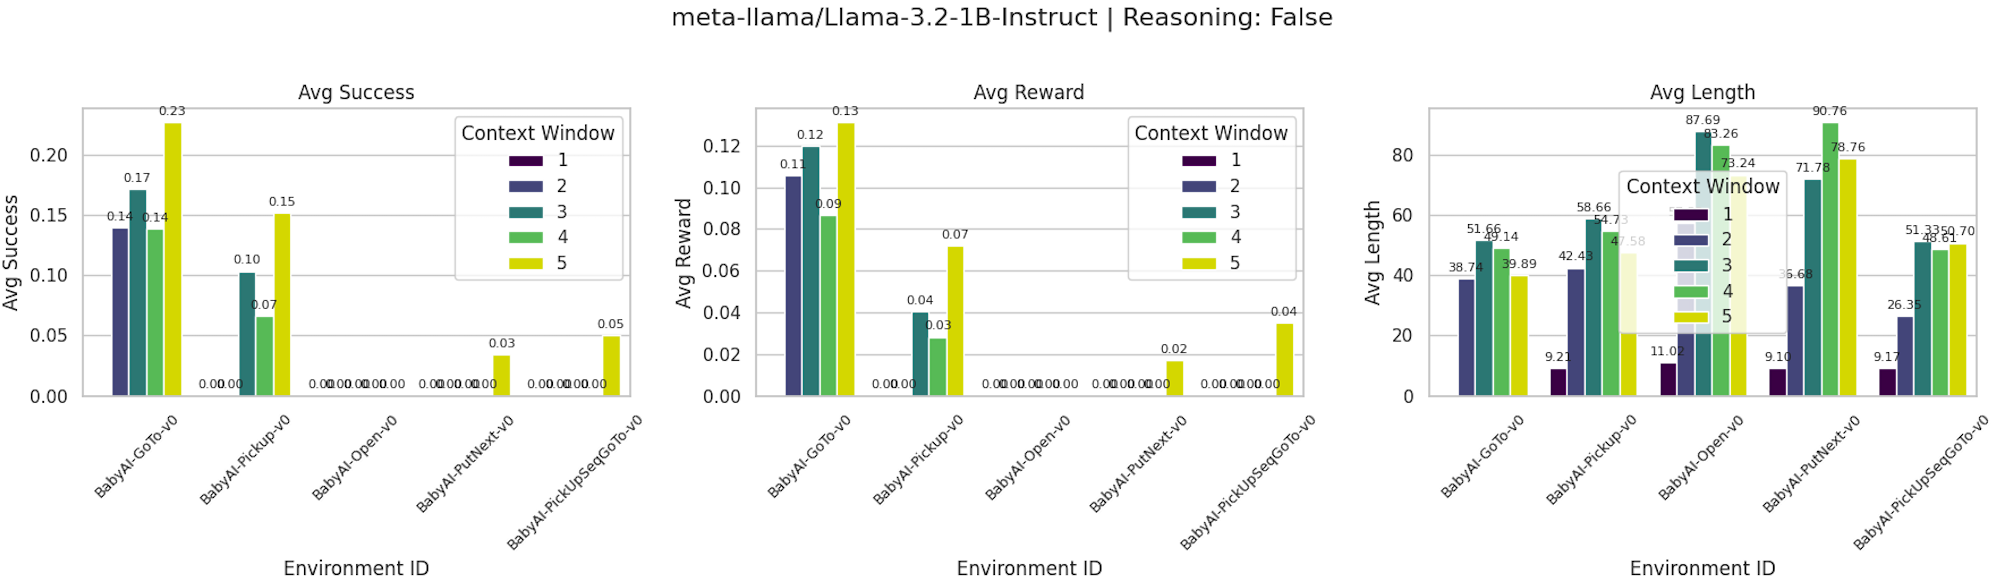
\includegraphics[width=1\linewidth]
    {../images/baseline_llama_1B_NR.png}
    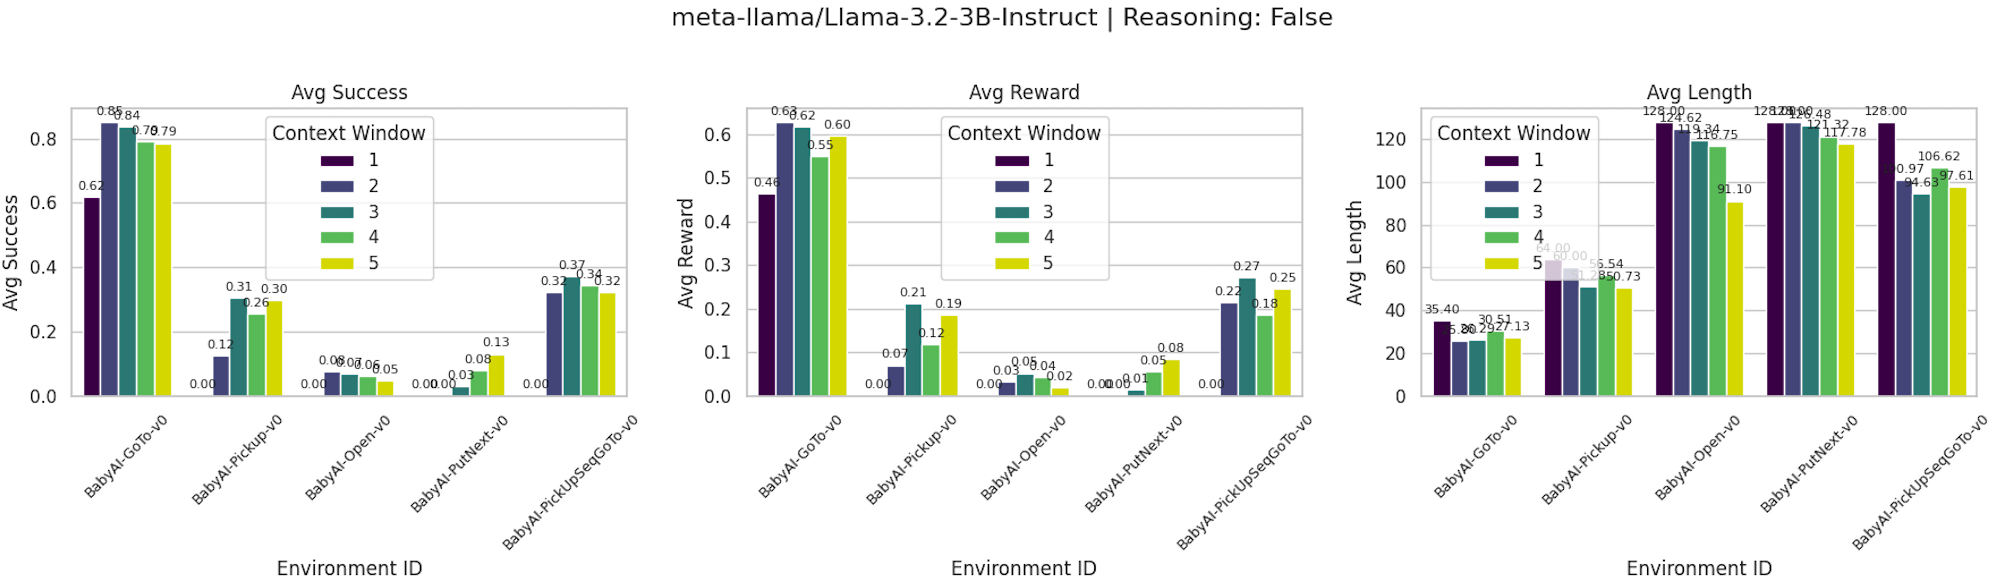
\includegraphics[width=1\linewidth]
    {../images/baseline_llama_3B_NR.png}
    \caption{Llama models under non-reasoning mode}
\end{figure}

\begin{figure}[H]
    \centering
    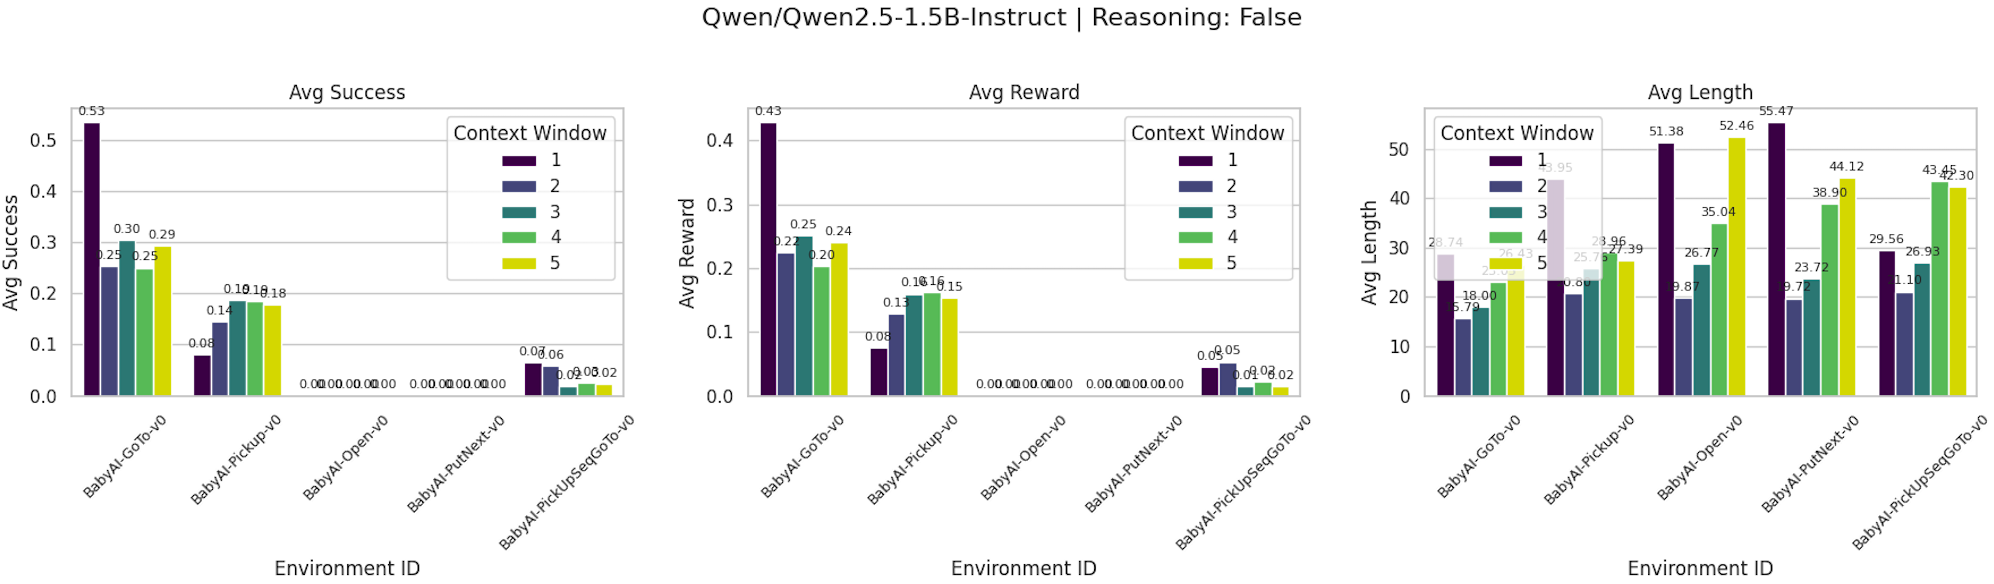
\includegraphics[width=1\linewidth]
    {../images/baseline_qwen_1.5B_NR.png}
    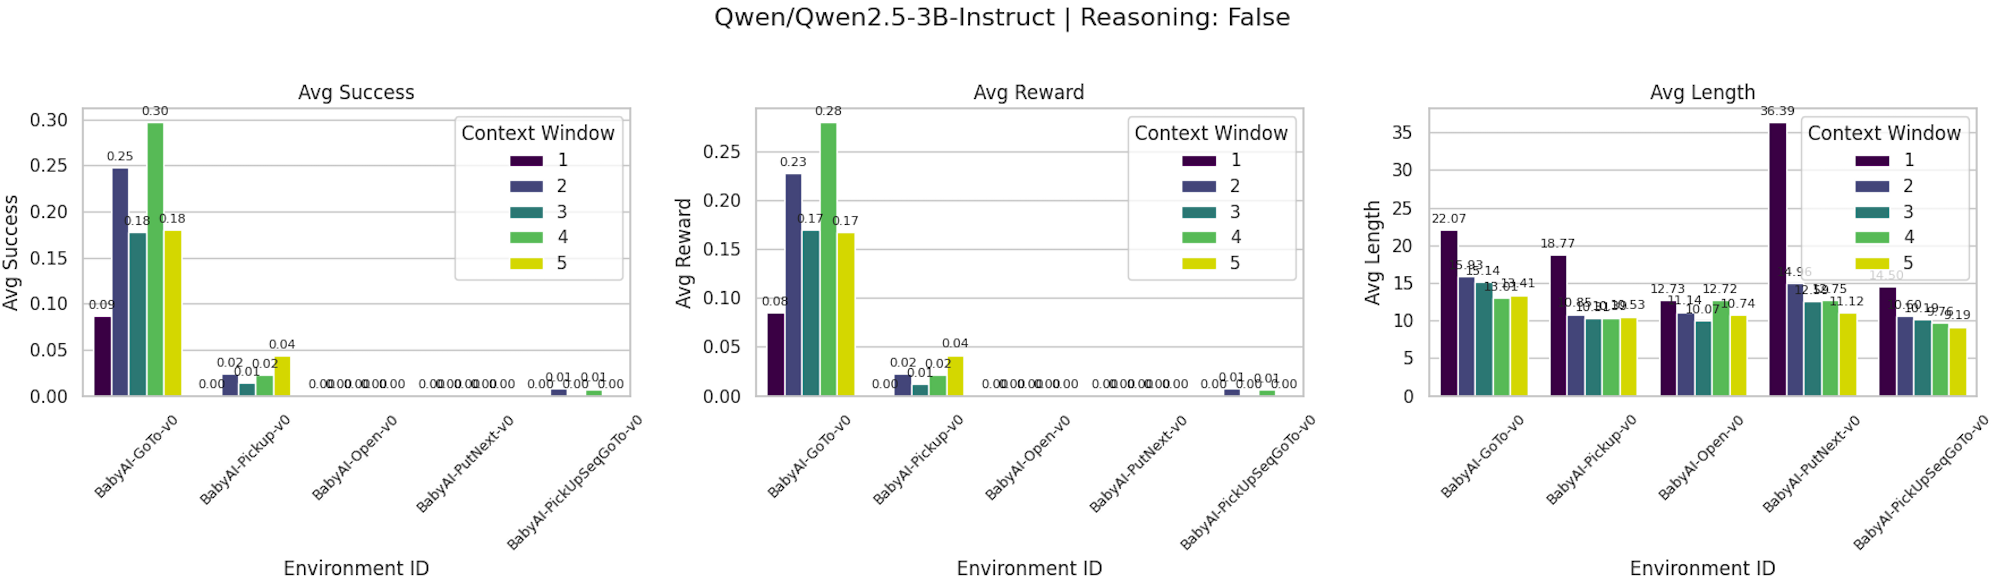
\includegraphics[width=1\linewidth]
    {../images/baseline_qwen_3B_NR.png}
    \caption{Qwen models under non-reasoning mode}
\end{figure}

\begin{figure}[H]
    \centering
    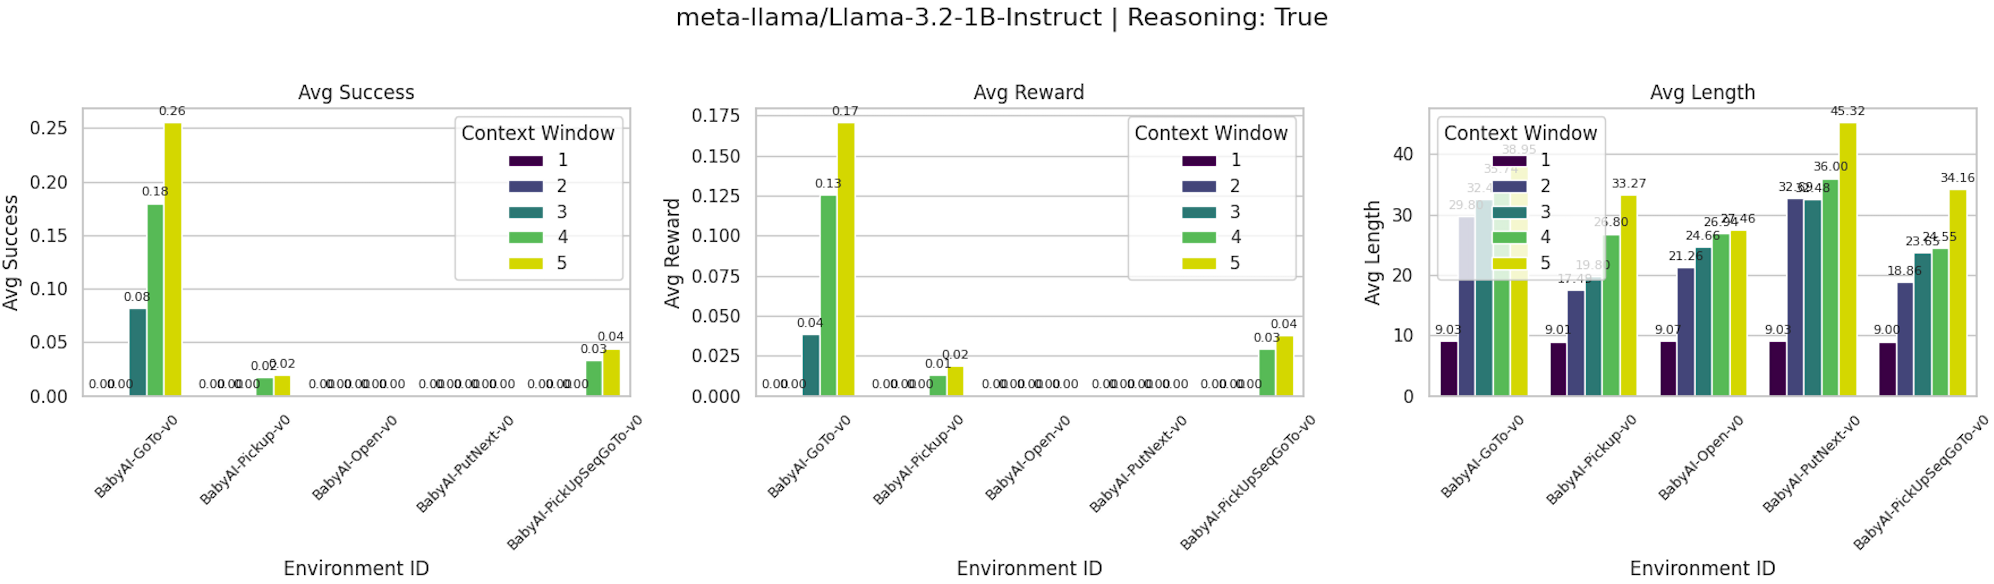
\includegraphics[width=1\linewidth]
    {../images/baseline_llama_1B_R.png}
    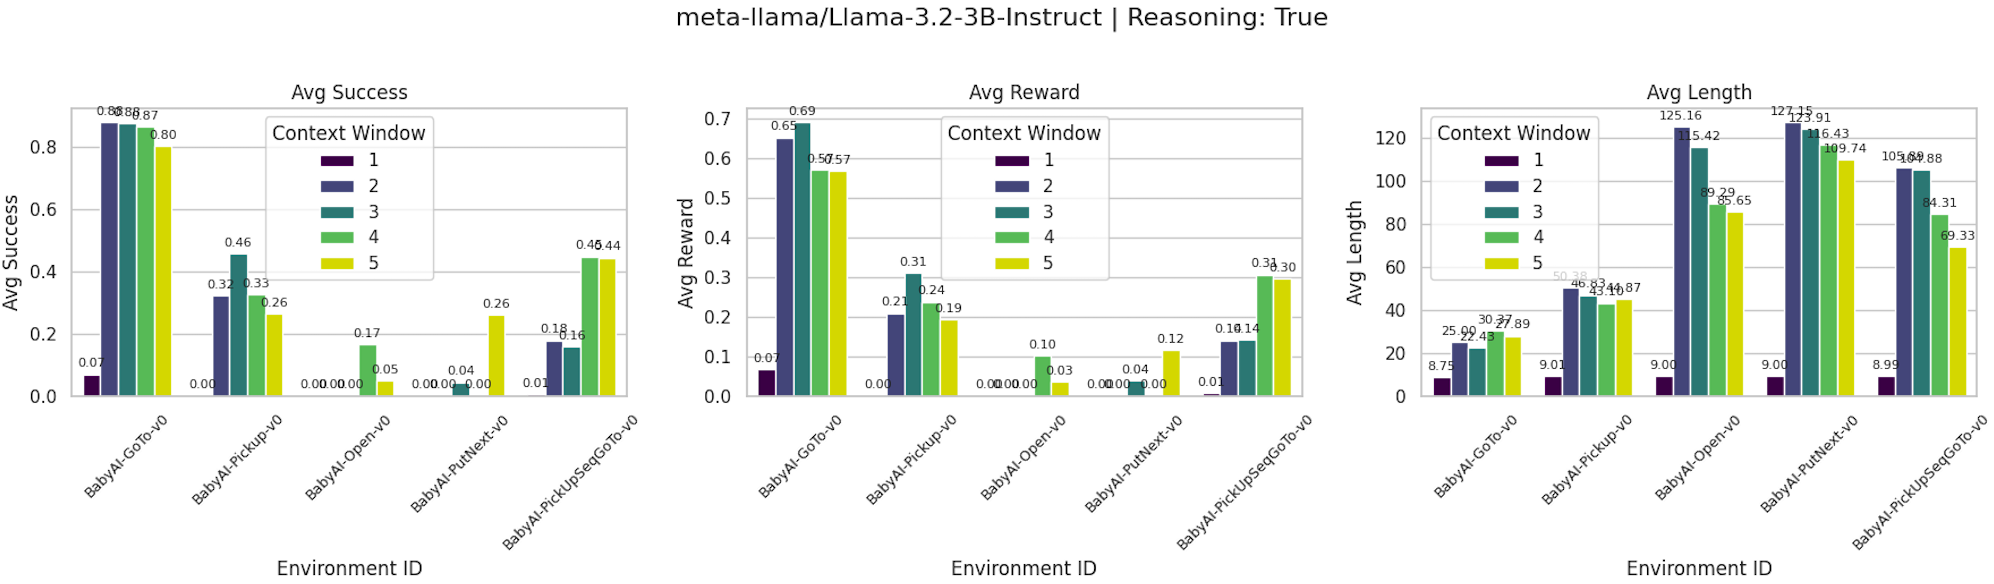
\includegraphics[width=1\linewidth]
    {../images/baseline_llama_3B_R.png}
    \caption{Llama models under reasoning mode}
\end{figure}

\begin{figure}[H]
    \centering
    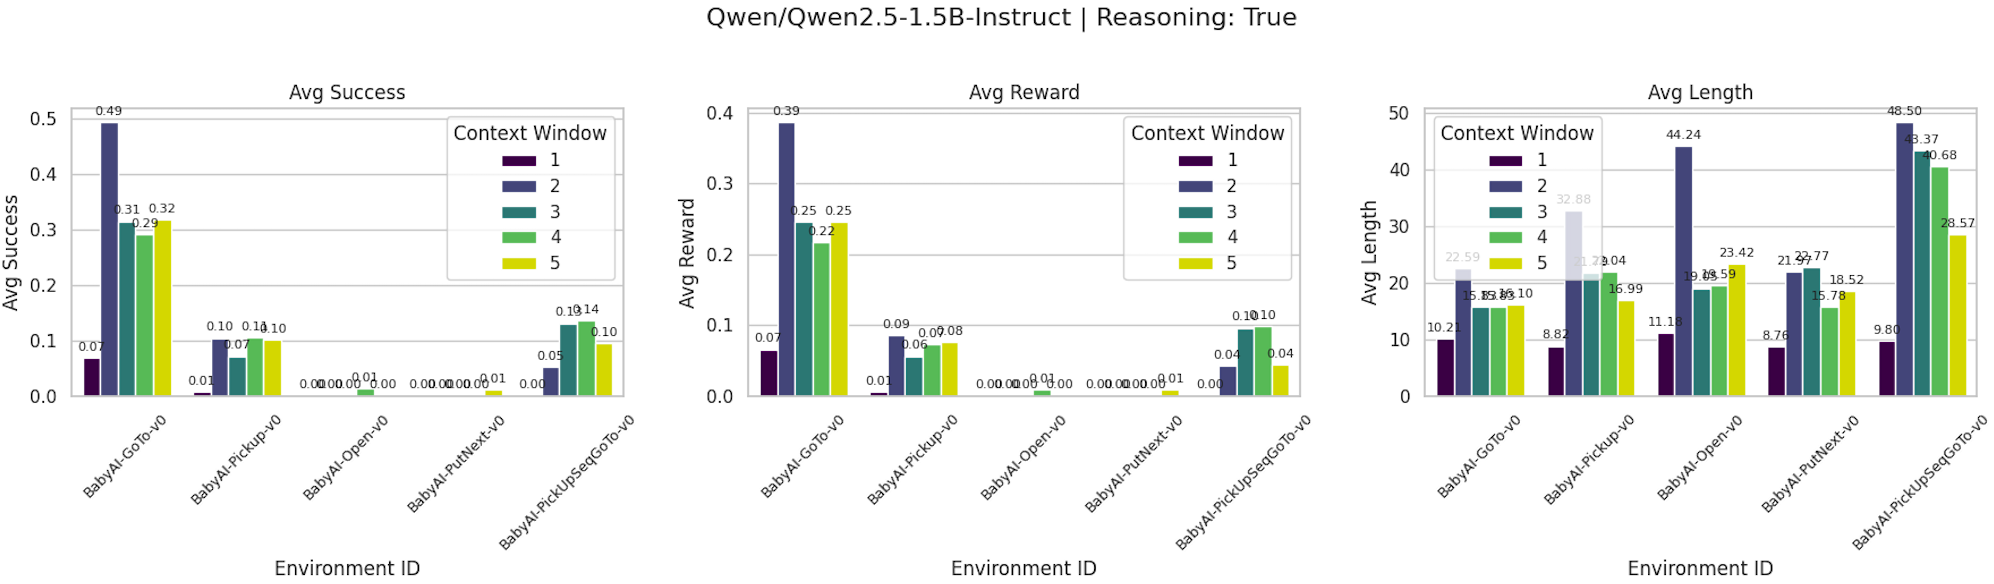
\includegraphics[width=1\linewidth]
    {../images/baseline_qwen_1.5B_R.png}
    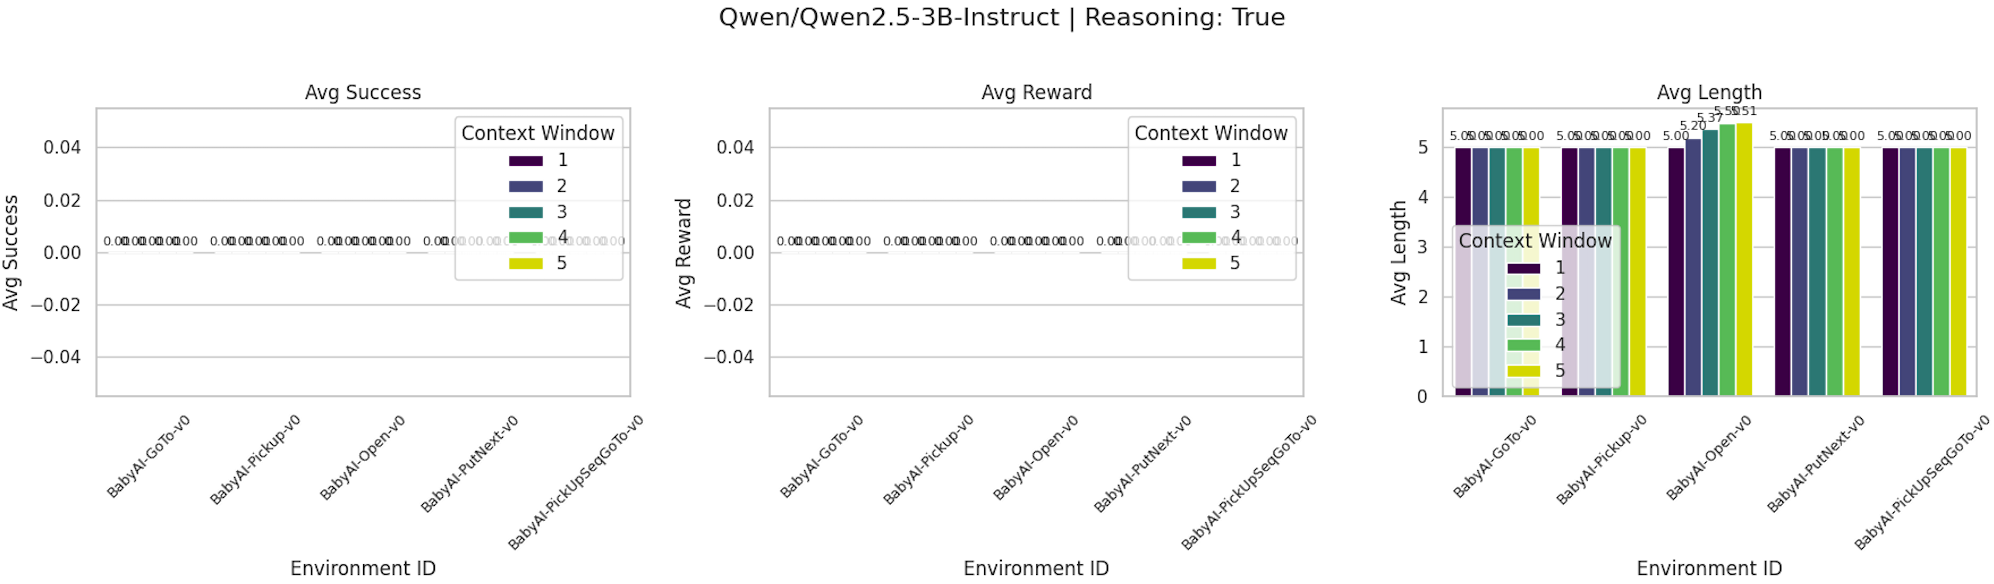
\includegraphics[width=1\linewidth]
    {../images/baseline_qwen_3B_R.png}
    \caption{Qwen models under non-reasoning mode}
\end{figure}

\newpage
\section{Contextual Bandit v.s. Nested PPO}
\label{appendix:ppo_comp}
We compare the average award and success rate on each batch for both algorithms. Nested PPO has better performance over contextual bandit in both non-reasoning and reasoning setups.

\subsection{Non-reasoning}
\begin{figure}[htbp]
    \centering
    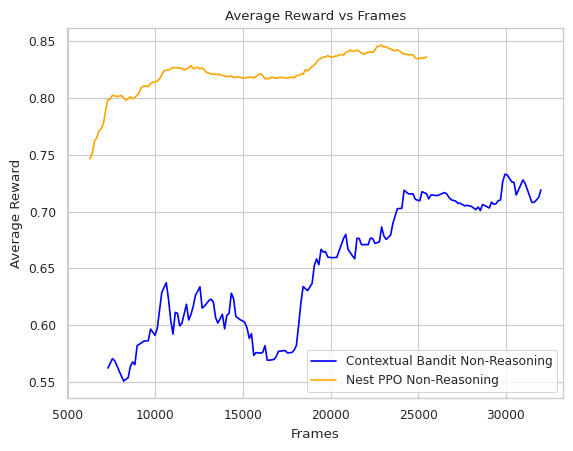
\includegraphics[width=0.6\linewidth]{../images/MC_TD_Reward_non_reasoning.png}
    \caption{Average Reward in Non-Reasoning Setup}
    \label{fig:mc_td_reward_nonreasoning}
\end{figure}

\begin{figure}[htbp]
    \centering
    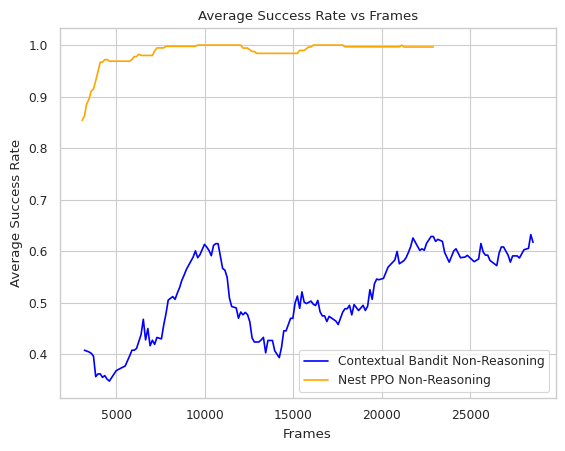
\includegraphics[width=0.6\linewidth]{../images/MC_TD_success_non_reasoning.png}
    \caption{Average Success Rate in Non-Reasoning Setup}
    \label{fig:mc_td_success_nonreasoning}
\end{figure}



\subsection{Reasoning}
\begin{figure}[htbp]
    \centering
    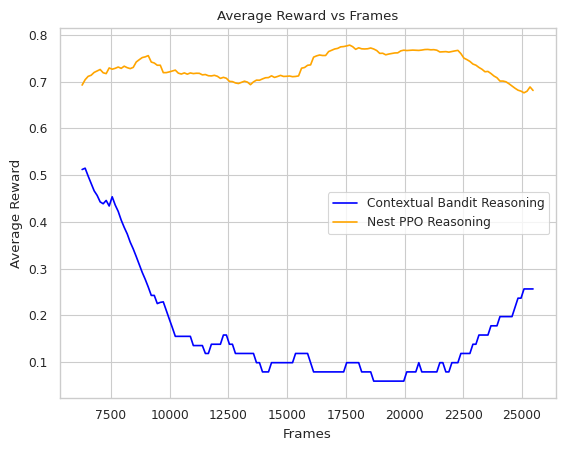
\includegraphics[width=0.6\linewidth]{../images/MC_TD_Reward_reasoning.png}
    \caption{Average Reward in Reasoning Setup}
    \label{fig:mc_td_reward_reasoning}
\end{figure}

\begin{figure}[htbp]
    \centering
    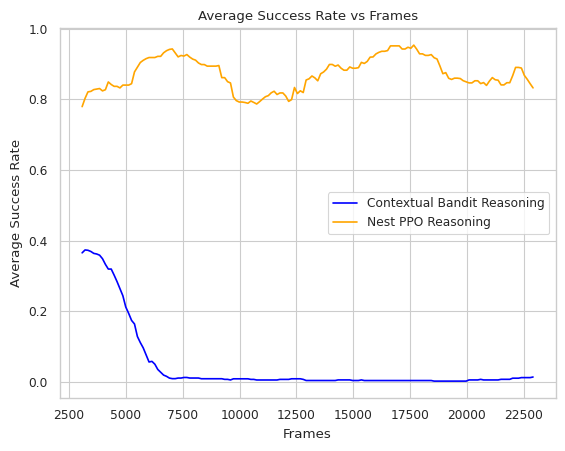
\includegraphics[width=0.6\linewidth]{../images/MC_TD_success_reasoning.png}
    \caption{Average Success Rate in Reasoning Setup}
    \label{fig:mc_td_success_reasoning}
\end{figure}

\newpage
\section{Hyperparameter Table}
\label{appendix:hyperparameter}
\begin{table}[htbp]
\begin{tabular}{|l|r|l|}
\hline
\textbf{Hyperparameter} & \multicolumn{1}{l|}{\textbf{Value}} & \textbf{Justification}                                       \\ \hline
num envs               & 6                                   & Parallel envs, subject to memory capacity                           \\
batch size             & 128                                 & Generated from current policy for policy update               \\
mini batch size       & 16                                  & For A100 GPU, this is the largest mini batch size we can use \\
learning rate          & 1.41E-05                            & Default in \texttt{TRL PPOTrainer}                                    \\
top k                  & 50                                  & Constrain the token space to avoid nonsense                  \\
top p                  & 0.9                                 &                                                              \\
temperature             & 0.7                                 &                                                              \\
Invalid action penalty  & -1                                  & Penalty if the generated action is not valid                 \\
early stopping         & \multicolumn{1}{c|}{TRUE}           & Stop the PPO optimization loop early is the KL too high.     \\
context window         & 5                                   & Trade-off between history queries and memory capacity        \\
$\gamma$                & 0.9                                 & Discount factor for trajectory return                        \\
$\lambda$               & 0.95                                & Decay factor for trajectory return                                                          \\
$\epsilon$              & 0.2                                 & Clip parameter in PPO                                                          \\
$\gamma_{\text{token}}$ & 1                                   & Discount factor for token GAE                                                             \\
$\lambda_{\text{token}}$& 0.98                                & Decay factor for token GAE                                                            \\ \hline
\end{tabular}
\caption{Hyperparameter List}
\end{table}

\newpage
\section{Training Curves}
\label{appendix: training-curves}
\begin{figure*}[htbp]
    \centering
    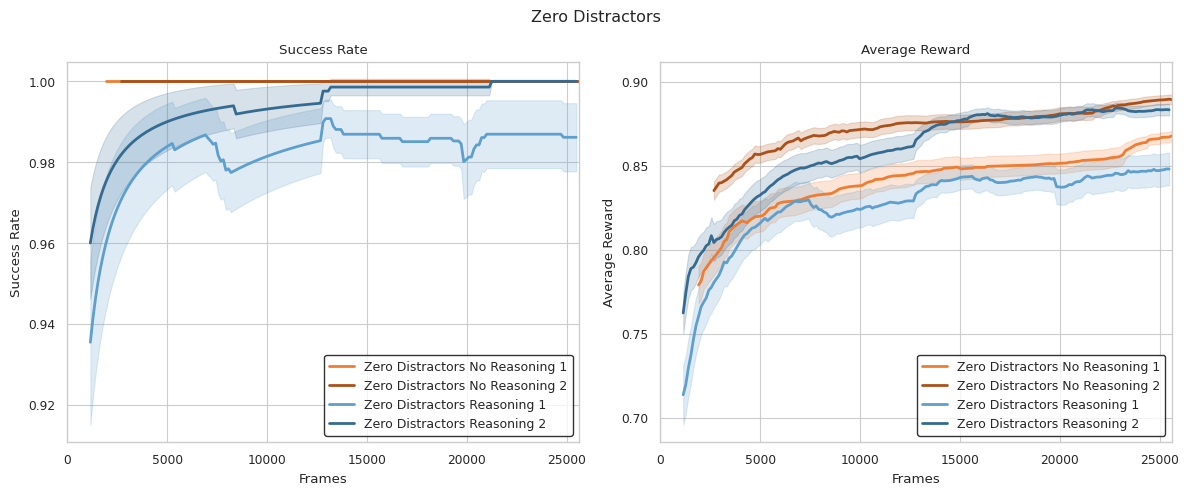
\includegraphics[width=\textwidth]{../images/zero_distractors_training_curves.png}
    \caption{Training curves for agents in environments without distractors.}
    \label{fig:no_distractors}
\end{figure*}
\begin{figure*}[htbp]
    \centering
    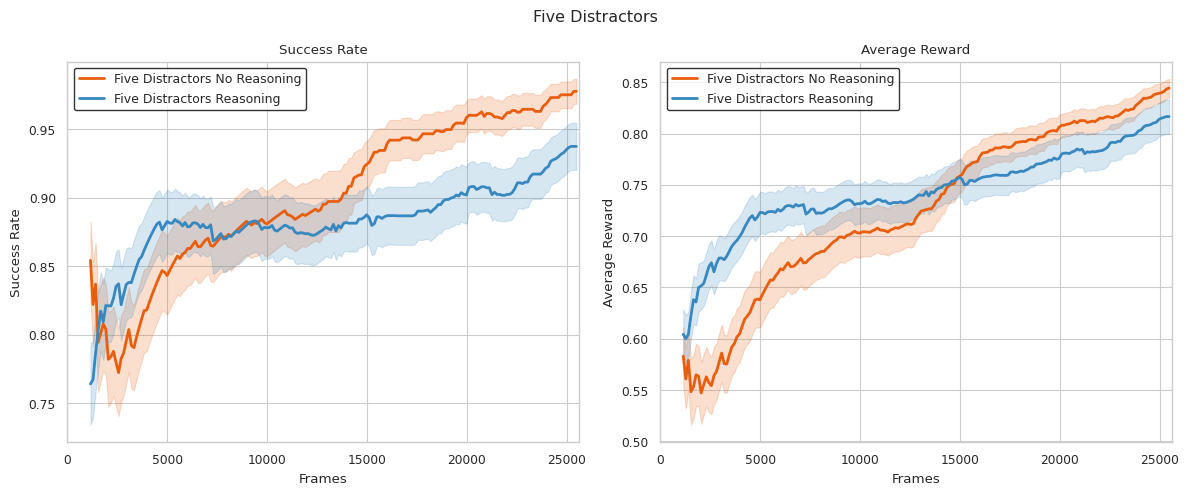
\includegraphics[width=\textwidth]{../images/five_distractors_training_curves.png}
    \caption{Training curves for agents in environments with five distractors.}
    \label{fig:five_distractors}
\end{figure*}


\newpage
\section{Evaluation Metrics}
\label{app:F}
The evaluation metrics on environment with 0 distractors are as follows:
\begin{table*}[htbp]
\centering
\scriptsize
\begin{tabularx}{\linewidth}{%
    l l
    >{\centering\arraybackslash}X 
    >{\centering\arraybackslash}X 
    >{\centering\arraybackslash}X 
    >{\centering\arraybackslash}X }
\toprule
\textbf{Env} & \textbf{Model Variant} 
& \textbf{Reasoning Success Rate $\pm$ Std} 
& \textbf{Non-Reasoning Success Rate $\pm$ Std} 
& \textbf{Reasoning Avg Reward $\pm$ Std} 
& \textbf{Non-Reasoning Avg Reward $\pm$ Std} \\
\midrule
\multirow{3}{*}{GoTo-v0} 
    & Zero-shot                & $0.66\pm0.48$ & $0.94\pm0.24$ & $0.55\pm0.41$ & $0.69\pm0.28$ \\
    & Zero-Distractor\_1      & $1.00\pm0.00$ & $1.00\pm0.00$ & $0.85\pm0.10$ & $0.91\pm0.05$ \\
    & Zero-Distractor\_2      & $1.00\pm0.00$ & $1.00\pm0.00$ & $0.90\pm0.07$ & $0.92\pm0.05$ \\
\midrule
\multirow{3}{*}{Pickup-v0} 
    & Zero-shot                & $0.64\pm0.48$ & $0.68\pm0.47$ & $0.47\pm0.39$ & $0.47\pm0.36$ \\
    & Zero-Distractor\_1      & $0.88\pm0.33$ & $1.00\pm0.00$ & $0.69\pm0.30$ & $0.85\pm0.10$ \\
    & Zero-Distractor\_2      & $1.00\pm0.00$ & $1.00\pm0.00$ & $0.88\pm0.06$ & $0.86\pm0.11$ \\
\midrule
\multirow{3}{*}{GoToTest-v0} 
    & Zero-shot                & $0.44\pm0.50$ & $0.96\pm0.20$ & $0.36\pm0.42$ & $0.75\pm0.23$ \\
    & Zero-Distractor\_1      & $0.98\pm0.14$ & $1.00\pm0.00$ & $0.82\pm0.18$ & $0.91\pm0.05$ \\
    & Zero-Distractor\_2      & $1.00\pm0.00$ & $1.00\pm0.00$ & $0.90\pm0.06$ & $0.92\pm0.05$ \\
\midrule
\multirow{3}{*}{PickupTest-v0} 
    & Zero-shot                & $0.72\pm0.45$ & $0.82\pm0.39$ & $0.53\pm0.36$ & $0.50\pm0.31$ \\
    & Zero-Distractor\_1      & $0.96\pm0.20$ & $1.00\pm0.00$ & $0.80\pm0.21$ & $0.87\pm0.10$ \\
    & Zero-Distractor\_2      & $1.00\pm0.00$ & $1.00\pm0.00$ & $0.87\pm0.06$ & $0.87\pm0.08$ \\
\bottomrule
\end{tabularx}
\caption{Summary statistics of zero-shot model and trained models on environments with 0 distractors}
\label{tab:performance0}
\end{table*}

The evaluation metrics on environment with 5 distractors are as follows:
\begin{table*}[htbp]
\centering
\scriptsize
\begin{tabularx}{\linewidth}{%
    l l
    >{\centering\arraybackslash}X 
    >{\centering\arraybackslash}X 
    >{\centering\arraybackslash}X 
    >{\centering\arraybackslash}X }
\toprule
\textbf{Env} & \textbf{Model Variant} 
& \textbf{Reasoning Success Rate $\pm$ Std} 
& \textbf{Non-Reasoning Success Rate $\pm$ Std} 
& \textbf{Reasoning Avg Reward $\pm$ Std} 
& \textbf{Non-Reasoning Avg Reward $\pm$ Std} \\
\midrule
\multirow{2}{*}{GoTo-v0} 
    & Zero-shot                & $0.46\pm0.50$ & $0.72\pm0.45$ & $0.33\pm0.39$ & $0.52\pm0.40$ \\
    & Five-Distractor          & $0.86\pm0.35$ & $1.00\pm0.00$ & $0.75\pm0.32$ & $0.88\pm0.13$ \\
\midrule
\multirow{2}{*}{Pickup-v0} 
    & Zero-shot                & $0.20\pm0.40$ & $0.32\pm0.47$ & $0.15\pm0.33$ & $0.21\pm0.34$ \\
    & Five-Distractor          & $0.86\pm0.35$ & $0.80\pm0.40$ & $0.74\pm0.32$ & $0.68\pm0.37$ \\
\midrule
\multirow{2}{*}{GoToTest-v0} 
    & Zero-shot                & $0.41\pm0.50$ & $0.90\pm0.30$ & $0.34\pm0.42$ & $0.63\pm0.31$ \\
    & Five-Distractor          & $0.88\pm0.33$ & $1.00\pm0.00$ & $0.79\pm0.30$ & $0.87\pm0.12$ \\
\midrule
\multirow{2}{*}{PickupTest-v0} 
    & Zero-shot                & $0.22\pm0.42$ & $0.30\pm0.46$ & $0.17\pm0.33$ & $0.22\pm0.36$ \\
    & Five-Distractor          & $0.82\pm0.39$ & $0.80\pm0.40$ & $0.72\pm0.35$ & $0.70\pm0.37$ \\
\bottomrule
\end{tabularx}
\caption{Summary statistics of zero-shot model and trained models on environments with 5 distractors}
\label{tab:performance5}
\end{table*}

We also include summary bar charts that resembles the evaluation metrics that can be found in Tables \ref{tab:performance0}, \ref{tab:performance3} and \ref{tab:performance5} for easy of readability and interpretability.

The plots for evaluation on environments with no distractors are as follows:
\begin{figure}[H]
    \centering
    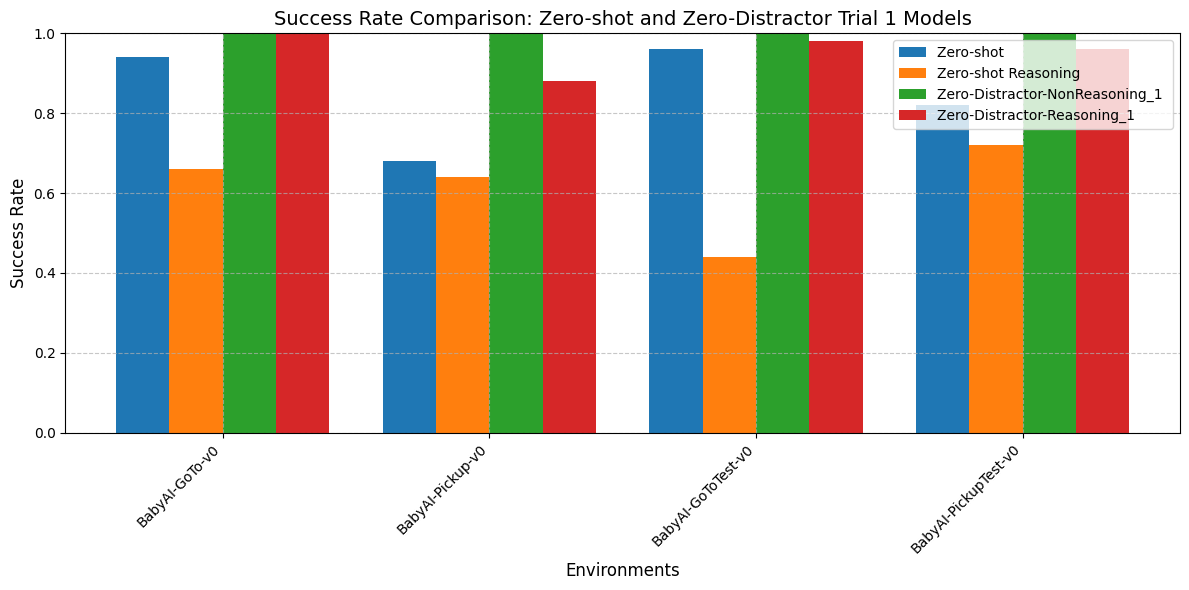
\includegraphics[width=1\linewidth]
    {../images/0-distractor-trial-1}
    \caption{Bar chart comparing zero-shot and first trained model performance in zero-distractor environments}
\end{figure}
\begin{figure}[H]
    \centering
    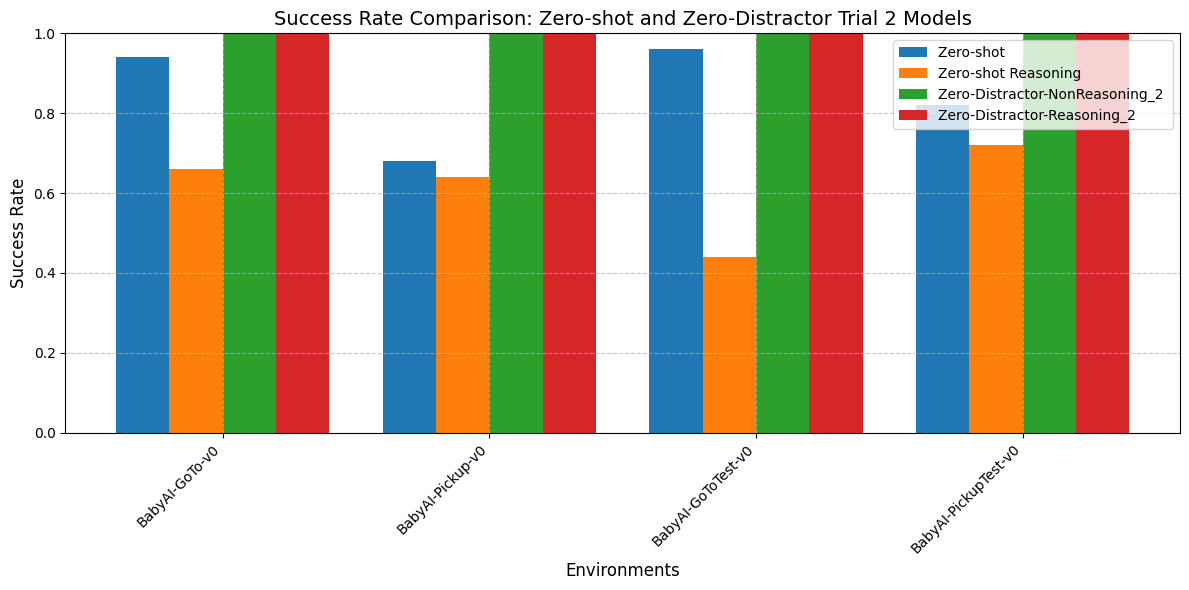
\includegraphics[width=1\linewidth]
    {../images/0-distractor-trial-2}
    \caption{Bar chart comparing zero-shot and second trained model performance in zero-distractor environments}
\end{figure}

\newpage
The plots for evaluation on environments with three distractors are as follows:
\begin{figure}[H]
    \centering
    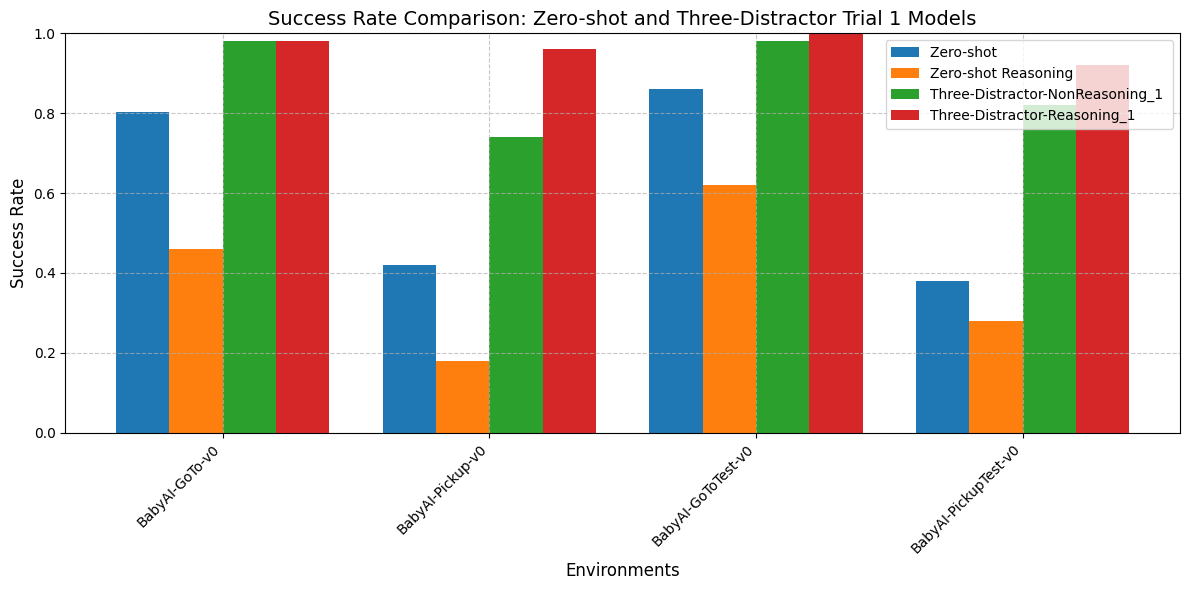
\includegraphics[width=1\linewidth]
    {../images/3-distractor-trial-1}
    \caption{Bar chart comparing zero-shot and first trained model performance in three-distractor environments}
\end{figure}
\begin{figure}[H]
    \centering
    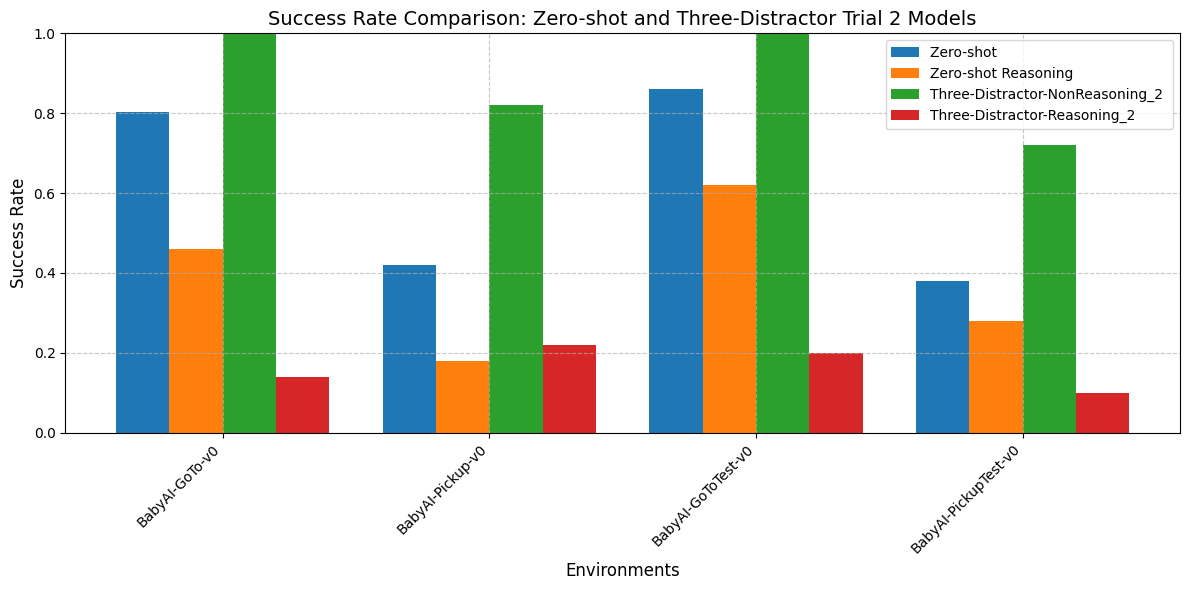
\includegraphics[width=1\linewidth]
    {../images/3-distractor-trial-2}
    \caption{Bar chart comparing zero-shot and second trained model performance in three-distractor environments}
\end{figure}
\newpage
The plot for evaluation on environments with five distractors is as follows:
\begin{figure}[H]
    \centering
    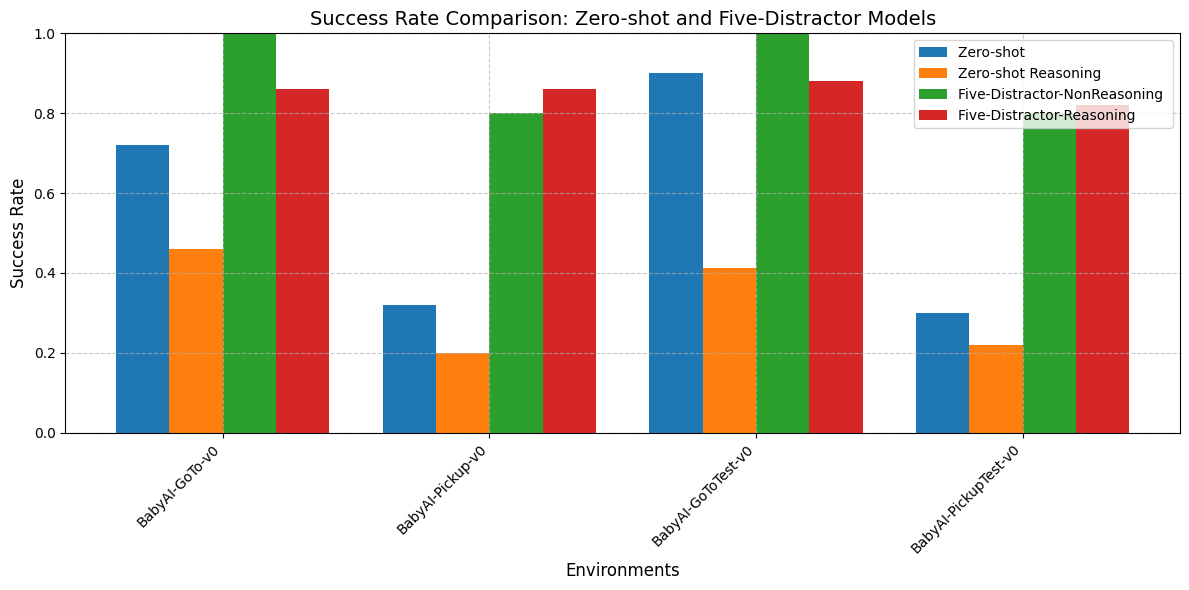
\includegraphics[width=1\linewidth]
    {../images/5-distractor}
    \caption{Bar chart comparing zero-shot and trained model performance in five-distractor environments}
\end{figure}

\newpage
\section{Model Performance on General Metrics}
\label{app:Z}
We evaluated model performance on two benchmarks unrelated to the BabyAI-Text environment, ARC-C and a subset of 1000 examples in HellaSwag. We discover that training the model under reasoning modes result in very similar performance to those trained under non-reasoning modes. In the below bar charts, we show performance of the model when trained under 1) no distractors; 2) three distractors and 3) five distractors, under reasoning and non-reasoning mode, respectively.

\begin{figure}[H]
    \centering
    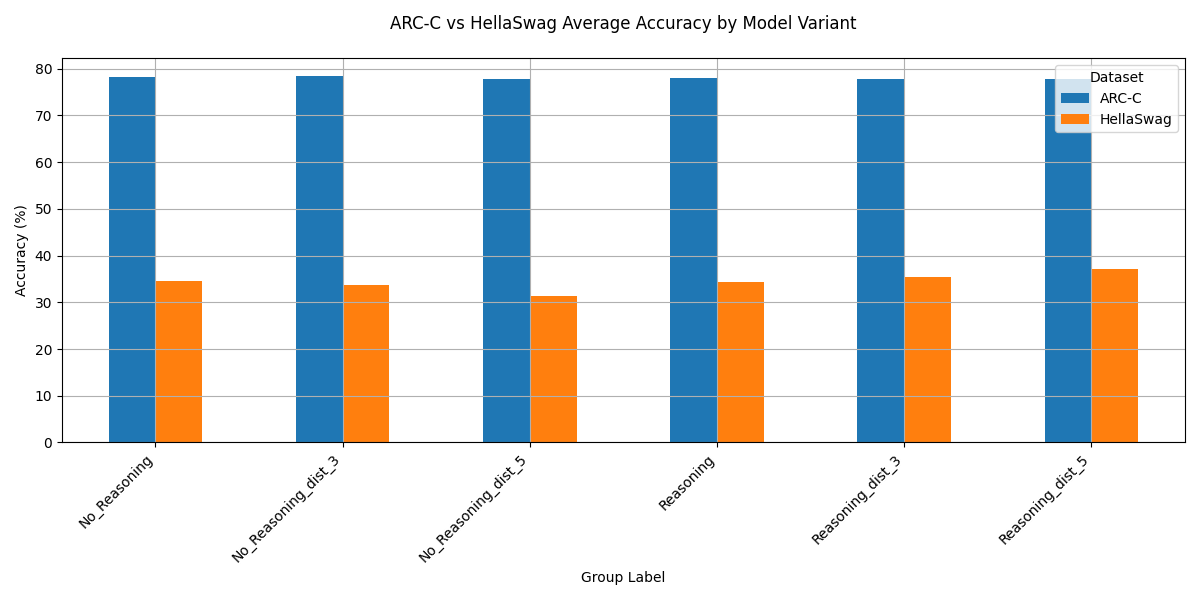
\includegraphics[width=1\linewidth]
    {../images/general_benchmark_plot.png}
    \caption{Model performance on general benchmarks}
\end{figure}

\newpage
\end{document}
